\documentclass[12pt,a4paper,oneside,openright,titlepage]{book}
\usepackage[utf8]{inputenc}
%\usepackage[italian]{babel}
\usepackage{amsmath,amscd}
\usepackage{amsfonts}
\usepackage{amssymb}
\usepackage{natbib}
\usepackage{braket}
\usepackage{caption} % 4 nice captions
\usepackage{amsmath}

\usepackage{bbm} %blackboard numbers


\usepackage{setspace} %per la copertina
\usepackage{graphicx} %per le immagini
\graphicspath{{images/}}



\usepackage{color}		% testo colorato
\usepackage[dvipsnames,table]{xcolor} % testo colorato & sfondo celle tabelle (rimelle)

\usepackage{hyperref}  %s

\usepackage{multirow} %multirow nelle tabelle

\usepackage{gnuplottex} %gnuplot

% SILLABAZIONE

\hyphenation{re-nor-ma-li-za-tion}
\hyphenation{o-pe-ra-tors}
\hyphenation{there-fore}
\hyphenation{li-te-ral-ly}
\hyphenation{cor-res-ponds}
\hyphenation{cor-res-pon-dence}
\hyphenation{cor-res-pon-ding}
\hyphenation{dy-na-mi-cal}
\hyphenation{i-ma-gi-na-ry}
\hyphenation{co-va-riant}
\hyphenation{mo-du-li}
\hyphenation{re-pre-sent-ed}
\hyphenation{phy-si-cal}
\hyphenation{the-o-ries}
\hyphenation{sub-ma-ni-fold}
\hyphenation{ma-ni-fold}
\hyphenation{me-tric}
\hyphenation{e-qui-va-lent-ly}



%STILE

\linespread{1.2}

% DICHIARAZIONI
% operatore traccia
\DeclareMathOperator{\Tr}{Tr}
%iperboliche

\DeclareMathOperator \ch {ch} 
\DeclareMathOperator \sh {sh} 

%volume

\DeclareMathOperator \vol {vol}

%pder
\newcommand{\pder}[2]{\frac{\partial#1}{\partial#2}}

%real im parts (must be AFTER amsmath, overrides it)
\renewcommand{\Re}{\operatorname{Re}}
\renewcommand{\Im}{\operatorname{Im}}

% string length
\newcommand{\strln}{\ell_s}
\newcommand{\onekten}{\frac{2\pi}{\strln^8}}
\newcommand{\hodge}{\ast}

% ibarj

\newcommand{\ibj}{i\bar{\jmath}}

%spinor conjugate
\newcommand{\scj}[1]{\overline{#1}}

%supersymmetry cursive N

\newcommand{\ssn}{\mathcal{N}}

%normal conjugate representation
\newcommand{\rrep}[1]{\mathbf{#1}}
\newcommand{\cjrep}[1]{\overline{\rrep{#1}}}

%mesonic moduli space
\newcommand{\mmes}{\mathcal{M}_\mathrm{mes}}

% Anti de Sitter
\newcommand{\ads}[1]{\operatorname{AdS}_{#1}}

%TIKZ

\usepackage{tikz}
\usetikzlibrary{arrows,decorations.markings,tikzmark}



%commenti in rosso
\newcommand{\cmmnt}[1]{\textcolor{Mahogany}{\emph{#1}}}


%\ref con parentesi





%FRONT
\author{Riccardo Antonelli}

\setlength\parindent{0pt}
\setlength{\parskip}{0.3cm} 
\begin{document}




\frontmatter


\begin{titlepage}
\begin{center}
 
% Upper part of the page

\includegraphics[scale=.5]{images/logoBlack}
 
\textsc{\LARGE Università degli Studi di Padova}\\[1.5cm]
 
\textsc{\Large Dipartimento di Fisica e Astronomia\\[0.2cm] Corso di Laurea Magistrale in Fisica}\\[2cm]
  
% Title

{\Huge \doublespacing \bfseries \begin{spacing}{1}{Holographic effective field theories: a case study}\end{spacing}}
~\\[4cm]
 
% Author and supervisor
\begin{minipage}{0.4\textwidth}
\begin{flushleft} \large
\emph{Laureando:}\\
Riccardo \textsc{Antonelli}
\end{flushleft}
\end{minipage}
\begin{minipage}{0.4\textwidth}
\begin{flushright} \large
\emph{Relatore:} \\
Luca \textsc{Martucci}
\end{flushright}
\end{minipage}
 
\vfill
 
% Bottom of the page
{\large Anno accademico 2015/2016\\
	\cmmnt{bozza compilata \today}}
 
\end{center}

\end{titlepage}

%\begin{frontespizio}
%\Universita{Padova}
%\Facolta{Scienze Matematiche, Fisiche e Naturali}
%\Corso[Laurea]{Matematica}
%\Titoletto{Tesi di laurea}
%\Titolo{Equivalenze fra categorie di moduli\\
%e applicazioni}
%\Candidato[145822]{Enrico Gregorio}
%\Relatore{Ch.mo Prof.~Adalberto Orsatti}
%\Annoaccademico{19??-19??}
%\end{frontespizio}

%\begin{abstract}

%\lipsum[1]

%\cmmnt{bozza compilata il giorno \today}\\

%\end{abstract}

\thispagestyle{plain}
\begin{center}
   % \Large
   % \textbf{Thesis Title}
    
   % \vspace{0.4cm}
   % \large
   % Thesis Subtitle
    
   % \vspace{0.4cm}
   % \textbf{Author Name}
    
   % \vspace{0.9cm}
    \textbf{Abstract}
\end{center}
%The identification of the low-energy effective field theory associated with a given microscopic strongly interacting theory constitutes a fundamental problem in theoretical physics, which is particularly hard when the theory is not sufficiently constrained by symmetries.
%Recently, a new approach has been proposed, which addresses this problem for a large class of four-dimensional minimally supersymmetric strongly coupled superconformal field theories, admitting a dual weakly coupled holographic description in string theory. This approach provides a precise prescription for the holographic derivation of the associated effective field theories. The aim of the thesis is to further explore this approach by focusing on a specific model, whose effective field theory has not been investigated so far. \cmmnt{(modificare abstract alla fine del lavoro.)}
The identification of the low-energy effective field theory associated with a given microscopic strongly interacting microscopic theory constitutes a fundamental problem in theoretical physics, particularly challenging when the theory is not sufficiently constrained by symmetries. Recently, a new approach has been proposed, which addresses this problem for a large class of four-dimensional minimally supersymmetric strongly coupled field theories, admitting a dual weakly coupled holographic description in string theory. This approach includes a precise prescription for the derivation of the associated effective theories through holography. The aim of this thesis is to explore these techniques by specializing them to a specific model whose effective theory has not been investigated before.


\tableofcontents

\mainmatter

\chapter{Introduction}

Strongly-coupled quantum field theories represent canonical examples of physical systems whose study is extremely challenging. Even the question of the mere existence of any interacting QFT in four dimensions from a formal standpoint has not been settled. In addition to this, strong couplings are not amenable to the tools of perturbation theory. The interest in this class of theories stems actually from practical considerations - many of them represent realistic models for physical phenomena, e.g. the theory of strong interaction.

A subset of questions concerns whether a given strongly-interacting theory is described at low energy by an effective local field theory, and if so, what are its degrees of freedom and their precise dynamics. Often, part of the structure of the effective theory is constrained by symmetries, but no general method exists to fix it completely. Recently \cite{MZ}, a novel approach for determining the effective Lagrangian was introduced that makes use of tools from an apparently unrelated area of physics: string theory.

It is remarkable that string theory was originally conceived as a description of hadronic physics, so a low-energy effective theory for what ultimately turned out to be a gauge theory, QCD. When string theory was found to have unsuitable qualities for this application, it was replaced by the theory of quantum chromodynamics - however it also proved to be effective for solving a seemingly unrelated problem of fundamental physics: quantizing gravity. Since then, string theory blossomed into a vast and rich field reaching into numerous areas of mathematics and physics, and of course a candidate for a ``Theory of Everything'' describing the entirety of fundamental physics.

Among the most unexpected discoveries in strings, made decades after their conception, is a series of unusual exact equivalences between string theories set in particular ten-dimensional backgrounds and four-dimensional gauge QFTs. More ge\-ne\-ral\-ly, one finds families of exact equivalences between local quantum field theories and higher-dimensional theories containing gravity, which are termed ``holographic''. This could be perhaps related to the original partial success of strings in modeling strong interactions, assuming that some or perhaps most gauge theories have or can be approximated as having a holographic description as a ten dimensional theory involving strings. This roundtrip has therefore brought strings back to strongly-coupled gauge theories. Various aspects, qualitative and most importantly quantitative, of QFTs can be studied directly by means of their holographic string dual, a gravitational theory, if it exists. 

The first and most important case of such a duality\cite{Maldacena} equates IIB superstring theory set on the background

\begin{equation}
	\operatorname{AdS}_5 \times \mathbb{S}^5
\end{equation}

(the ``bulk'') with maximally supersymmetric Yang-Mills theory on $\mathbb{R}^{1,3}$ (the ``boun\-da\-ry''), which is a conformal field theory. The denomination of ``AdS/CFT'' (anti-de Sitter / conformal field theory) correspondence for holographic dualities stems from this (even though cases either with no AdS geometry or not conformal are known). One direction in which to generalize this construction is to replace $\mathbb{S}^5$ with other compact 5-manifolds $Y_5$. This yields dualities involving more complex and interesting field theories, less constrained by symmetries; therefore this thesis will be focused on this class of correspondences.

Actually, since string theory in general is very challenging to study, AdS/CFT only becomes truly useful in terms of describing the dynamics of the CFT if string theory can be approximated by a weakly coupled effective field theory of its own, supergravity. This limit corresponds to the CFT being strongly-coupled and having a large number of colours. Therefore the regime accessible through holography is precisely the strongly-coupled region where the gauge theory would be normally impossible to investigate.

Recently, a novel approach was introduced\cite{MZ} for determining the effective theory to such duals of $\operatorname{AdS}_5 \times Y_5$. A procedure for identifying the degrees of freedom and the Lagrangian for the effective low-energy theory for a class of gauge theories with $\operatorname{AdS_5} \times Y_5$ holographic duals is provided, by expanding the supergravity action on the dual bulk geometry. Interestingly, these are somewhat special in that they include models of minimal supersymmetry ($\mathcal{N}=1$), which makes for more realistic but by converse less constrained theories than typical holographic field theories, with higher supersymmetry. The ability to pinpoint the exact effective Lagrangian is then particularly noteworthy.

The original contribution in this work is the specialization of this construction to a specific field theory, the $Y^{2,0}$ theory, a strongly-coupled superconformal quiver theory for which we will therefore fix the exact effective Lagrangian, entirely through the geometry of the relative string background. This will require necessarily the determination of the general Calabi-Yau deformation of the background in complex coordinates, which was not known previously.

This thesis will be structured as follows. We will first provide a general introduction to IIB superstring theory, D-brane stacks on cones and the resulting gauge field theories, and holography. Then, we will summarize the relevant results and techniques from \cite{MZ}. Finally, we will present a complete parametrization of the geometry of the $Y^{2,0}$ theory and will apply those results and techniques to identify the exact effective Lagrangian of the field theory.



\chapter{IIB superstrings and branes}

String theories are quantum theories involving 1-dimensional dynamical objects, the fundamental strings. Therefore, they can be regarded as a generalization of systems of 0-dimensional quantum particles, such as quantum field theories. This apparently innocuous modification results in amazing depth and complexity of the structure of the resulting theories. The celebrated inclusion of Einstein gravity is only a small part of the large diversity of phenomena. 

The downside is a significant difficulty in probing the general structure of these theories. Only the behaviour in particular regimes is known, while the overall theory interpolating between these limiting cases is mostly unknown, or at the very least impossible to formulate. Consequently, we will only attempt an introduction to the aspects of string theory relevant to our purposes, namely when strings can be approximated by an effective field theory (and which one), and stable non-perturbative states known as D-branes.

Our interest will be directed towards string theories involving supersymmetry, and in particular a particular variety known as type IIB string theory, set in ten dimensions, which will always be involved in the holographic dualities we will study. In fact, IIB will be both the background theory employed to construct the holographic duality, and one side of the duality itself. Thus, we now provide a summary starting from perturbative superstring theory to present some general aspects of type-IIB strings, including the corresponding effective field theory and D-branes.

\section{Superstring theory}

String theory either does not admit a nonperturbative Lagrangian formulation, or this formulation is unknown. An action functional can only be written upon choosing a perturbative vacuum; since we anticipate a string theory must include gravity, a choice of vacuum will also require a choice of background metric - in the simplest case Minkowski spacetime. The configuration of a string moving in this spacetime (the target $M$) is then given by specifying the two-dimensional submanifold (the worldsheet $W_1$) it traces in it\footnote{We note the worldsheet is just the obvious generalization of the concept of worldline of a particle to the case of 1-dimensional strings.}, the worldsheet. In essence, this coincides with providing an embedding of the worldsheet

\begin{equation}
	X^{\mu} (\tau,\sigma) : W_1 \rightarrow M
	\label{}
\end{equation}

then quotiented under diffeomorphisms of the coordinates $\tau,\sigma$ on $W_1$.

With a given choice of background metric the most natural action for a string is the Nambu-Goto action, the worldsheet area:

\begin{equation}
	S_{NG}\left[ X \right] = - T \int_{W^1} d\vol_h = - T \int_{W^1} d^2 \sigma \sqrt{-h}
	\label{}
\end{equation}

where $h_{ab} = \pder{x^\mu}{\sigma^a} \pder{x^\nu}{\sigma^b} G_{\mu\nu}$ is the induced metric on the worldsheet from the target space metric $G_{\mu\nu}$ under the embedding given by $X^\mu$. $T$ instead is a dimensionful constant called the string tension; in fact it is the only free parameter in string theory. We will also often refer to the entirely equivalent quantity $\alpha'$, the Regge slope. \cmmnt{check convenzioni!}

\begin{align}
	T = \frac{1}{2\pi\alpha'}
	\label{}
\end{align}

The Nambu-Goto action is very difficult (if not impossible) to quantize. It proves much easier to switch to the classically equivalent Polyakov action: 

\begin{equation}
	S_B\left[ X,g \right] = -\frac{T}{2} \int_{W^1} d^2\sigma \sqrt{-g} g^{ab} \partial_a X^\mu \partial_b X_\nu G_{\mu\nu}
\end{equation}

%where the $D$ fields $X^\mu$ describe the embedding of the string's worldsheet in the $D$-dimensional target spacetime, and the integral is performed over the worldsheet coordinates $\sigma^a = (\tau,\sigma)$. The $X^\mu$ are of course scalars from the point of view of the worldsheet. The auxilary field $g_{ab}$ is a metric on the worldsheet. 

where now $g_{ab}$ is an independent auxiliary field, not the induced metric from the $X^\mu$. The equivalence is readily shown by computing the classical equation of motion for $g_{ab}$ and substituting back into $S_B$ to recover $S_{NG}$.


There are essentially two\footnote{We ignore the question of orientability of the worldsheet, not important for our purposes.} different sensible choices for the topology of $W_1$: either a cylinder, with $\sigma$ being the periodic variable running around, or a strip, so that $\sigma$ is limited to an interval $[0,\sigma_1]$. These are respectively the closed and open string. The former is always a closed loop at any given instant in time. The open string instead has two endpoints for which we have to fix boundary conditions.  One could choose between either Neumann boundary conditions, meaning

\begin{equation}
	\left. \pder{X^\mu}{\sigma}\right|_{\sigma = 0,\sigma_1} = 0
	\label{}
\end{equation}

which is just the constraint that no momentum flows out of the string endpoints, or Dirichlet boundary conditions, which fix 

\begin{align}
	\left. X^\mu \right|_{\sigma=0} = X_0^\mu, && \left. X^\mu \right|_{\sigma=\sigma_1} = X^\mu_{\sigma_1}
	\label{}
\end{align}

where $X^\mu_0$, $X^\mu_{\sigma_1}$ are constants, essentially forcing the string endpoints to a specific spacetime point. In general one could mix $p+1$ Neumann conditions and $D-p-1$ Dirichlet conditions for different values of $\mu$, so that the endpoints are constrained to a $p$-dimensional submanifold in space, and can move freely within it. Dirichlet conditions evidently break the symmetries of the target spacetime (Poincar\'e if we choose a Minkowski background) as they specify a preferential frame and submanifold; this symmetry will be recovered when it is recognized that the $p$-dimensional submanifold to which open strings attach is actually a dynamical object, a D$p$-brane (D alluding to Dirichlet). We will return to D-branes after studying the string spectrum.

The Polyakov action displays invariance under worldsheet diffemorphisms 

\begin{equation}
	\sigma_a \rightarrow \sigma_a'(\sigma_a)
	\label{}
\end{equation}

and Weyl transformations:

\begin{equation}
	g_{ab} \rightarrow e^{\phi(\sigma)} g_{ab} 
	\label{}
\end{equation}

and thus perturbative string theory is naturally a two-dimensional conformal field theory. These symmetries must be quotiented out someway on quantization. The most straightforward way is to eliminate them by fixing a particular gauge and then quantizing (canonical quantization). The three symmetry generators can kill the three degrees of freedom in the metric to fix it to the 2D Minkowski: $g_{ab} = \eta_{ab}$. We get

\begin{equation}
S_B = - \frac{T}{2} \int d^2\sigma \partial_a X^\mu \partial^a X_\mu
\end{equation}

where indices are raised with $\eta^{ab}$.

The theory described so far would be what is known as bosonic string theory. There are two issues with bosonic strings: the first is the presence of tachyons in both the open and closed string spectrum, i.e. some string modes will have a negative mass squared, signaling an instability of our choice of perturbative vacuum. The second is that, as the name suggests, there are exclusively bosons in the spectrum, which makes it unsuitable at the very least for phenomenological application. A modification to include supersymmetry can be performed to solve both of these issues and produces a set of string theories with fermions and without tachyons, the superstrings. We will in particular sketch the path from bosonic string theory to the so-called type II superstrings, two slightly different theories IIA and IIB.

There are at least two different approaches to introducing supersymmetry into a string theory. The path followed by the RNS (Ramond-Neveu-Schwarz) formalism is to impose SUSY at the worldsheet level; explicitly, adding fermions $\psi^\mu$ to act as superpartners to the bosons $X^\mu$. We follow the derivation in \cite{BBS}. The action is extended to

\begin{equation}
S = S_B + S_F = -\frac{T}{2} \int d^2\sigma \; \partial_a X^\mu \partial^a X_\mu + \bar \psi^\mu \rho^a \partial_a \psi_\mu
\end{equation}

where the $\rho^{1,2}$ are two-dimensional gamma matrices satisfying the Clifford algebra

\begin{equation}
	\left\{ \rho^a,\rho^b \right\} = 2\eta^{ab}
	\label{}
\end{equation}

The spinors' equation of motion, the Dirac equation, is actually the Weyl condition in two dimension. This brings the real degrees of freedom in the spinor for each $\mu$ from $4$ to $2$. Recalling that in $(2\bmod 8)$ dimensions there exist Weyl-Majorana spinors satisfying both the Weyl and Majorana conditions, imposing the latter on $\psi$ halves again the on-shell polarizations to $1$. Thus we have a match between bosonic and fermionic degrees of freedom. It can be proven\cmmnt{(ref)} the theory above is indeed worldsheet supersymmetric.

To quantize canonically, we introduce canonical commutation/anticommutation relations:

\begin{align}
[X^\mu(\sigma),X^\nu(\sigma')] = \eta^{\mu\nu} \delta^2(\sigma-\sigma') && \{\psi^\mu(\sigma),\psi^\nu(\sigma')\} = \eta^{\mu\nu} \delta^2(\sigma-\sigma')
\end{align}

Note the $X^0$ and $\psi^0$ would create negative norm states, but these modes are eliminated by resorting to superconformal invariance. Classically this symmetry imposes the stress-energy tensor $T^{\mu\nu}$ and the supercurrent $J^a_\alpha$ vanish; imposing that in the quantum theory they annihilate physical states yields the restriction that removes the longitudinal ghosts from the spectrum. These take the name of super-Virasoro constrain.

Then the procedure for building the string spectrum is to expand the classical solutions in terms of Fourier modes, identify creators and destructors, and then select the states of the Fock basis that satisfy the super-Virasoro constraints. There are various ways to proceed at this point; the simplest and perhaps the most inelegant is light-cone quantization, which we will refer to. Essentially, a subset of $D-2$ transverse directions $i=2,\ldots,D-1$ are selected and only $X^i$ and $\psi^i$ are made to correspond to operators, and the remaining longitudinal fields are to be determined from the former by the classical constraints. This procedure renders Lorentz-invariance non-manifest - we will verify indeed it is actually recovered a posteriori. A different common approach, more rigorous, takes the form of a BRST quantization, akin to that employed in Yang-Mills theories, by exchanging superconformal gauge invariance with the introduction of a series of Faddev-Popov ghosts. The final quantum theories are identical and the choice of quantization is conventional.

Boundary conditions for $\psi^\mu$ for an open string can actually be satisfied in two different by imposing periodicity or antiperiodicity, giving rise to the NS (Neveu-Schwarz) and R (Ramond) sectors, built over two grounds $\ket{0}_{NS}$ and $\ket{0}_R$. Closed strings have four: $\ket{0}_{NS-NS}$, $\ket{0}_{R-R}$, $\ket{0}_{R-NS}$, $\ket{0}_{NS-R}$ corresponding with different choice periodicity conditions for left and right-movers.

\subsection{Open strings}\label{sec:openstring}

It can be shown that while the NS ground $\ket{0}_{NS}$ is unique, and thus a spacetime scalar, $\ket{0}_R$ is eight-fold degenerate and this 8-plet transforms under the spinor representation of transverse $SO(8)$ - in other words, it is a spacetime spinor. In particular, it is a chiral Weyl-Majorana spinor, so it can be taken to be either of positive or negative chirality, choices we will denote as $\ket{+}^a_R$, $\ket{-}^{\dot a}_R$, with $a,\dot{a}=1,\ldots,8$ the spinor index.

The spectrum is built by acting on one of the grounds with bosonic and fermionic creators, to obtain states of higher and higher mass. For the NS sector, there are bosonic creators $a_n^{i\dagger}$ ($n\geq 1$) and fermionic $b_r^{i\dagger}$ ($r$ positive half-integer), and the mass of the excited string is given by:

\begin{equation}
	\alpha' M^2 = \sum_{n=1}^\infty n \,a_n^{i\dagger} a_n^i  + \sum_{r=1/2}^\infty r b_r^{i\dagger} b_r^i - \frac{1}{2}
	\label{massshellNS}
\end{equation}

while for the R sector the fermionic creators are replaced by the integer-indexed $d_n^{\dagger i}$:

\begin{equation}
	\alpha' M^2 = \sum_{n=1}^\infty \left(n\, a_n^{i\dagger} a_n^i + n d_n^{i\dagger} d_n^i \right)
	\label{massshellR}
\end{equation}

The $i$ indices here are target spacetime transverse indices, $i=1,\cdots,8$. Therefore each creator increases the spacetime spin of the string by one unit. We conclude the NS sector contains only spacetime bosons, and the R sector only spacetime fermions.

The constant shift of $-1/2$ in \eqref{massshellNS} (and of $0$ in \eqref{massshellR}) actually results from an ordering ambiguity of the creators and destructors $a_n^\dagger$, $a_n$ (omitting spacetime indices for now) which introduces an arbitrary constant shift in the Hamiltonian upon quantization. If we want a consistent quantum theory with Lorentz invariance, this shift in the NS sector is fixed to $-1/2$; this is because for example the state

\begin{equation}
	b_{1/2}^{i\dagger} \ket{0}_{NS}
	\label{}
\end{equation}

is a vector with $(D-2)$ polarizations, and thus must be massless. However, it can be shown that this shift is also related to the number of spacetime dimensions $D$, so that a condition restricting $D$ to a particular value can be found. An intuitive and perhaps heuristic explanation of this fact is as follows: the energy shift should be equal to the sum of the zero-point energies (ZPE) of the infinite harmonic oscillators, bosonic for $n = 1, 2, \ldots $  and fermionic for $r= 1/2, 3/2, \ldots$ We recall bosonic / fermionic QHOs have Hamiltonians

\begin{align}
	H = \omega \left( a^\dagger a + \frac{1}{2} \right) && H = \omega \left( b^\dagger b - \frac{1}{2} \right)
	\label{}
\end{align}

Then for a given value of $i$ the sum of all the ZPEs of the oscillators in the NS sector would be

\begin{equation}
	E_0 =	\sum_{n\in \mathbb{N}} \frac{n}{2} \,- \sum_{r \in \mathbb{N}+\frac{1}{2}} \frac{r}{2} = \frac{1}{4} \sum_{m \in \mathbb{N}} (-1)^m m
	\label{}
\end{equation}

The sum $-1 + 2 - 3 + \ldots$ is evidently divergent; we assume it is admissible to replace it with its $\zeta$-regularized value\footnote{The evaluation by analytic continuation of the divergent series is easily computed by considering $1-2x + 3x^2 - \ldots = (1+x)^{-2}$, converging for $|x|<1$. Setting $x=1$, right on the edge of the disk of convergence, yields the desired result.} of $-1/4$. Therefore the ZPE per transverse direction is $E_0 = -1/16$; insisting the total ZPE is equal to $-1/2$ results in

\begin{equation}
	-\frac{D-2}{16} = -\frac{1}{2} \Rightarrow D = 10
	\label{}
\end{equation}

While this argument is not completely rigorous, it correctly identifies the existence and value of the so called critical dimension $D=10$ for superstring theories. In a more formal setting (e.g., in BRST quantization) it can be shown that the classical Weyl symmetry of the action is spoiled by quantization and a conformal anomaly arises; this anomaly can be proven to cancel\footnote{it is possible to have the conformal anomaly cancelled by the introduction of additional fields if $D<10$, resulting in non-critical string theories. These have properties that make them unsuitable for our applications, however, and we will ignore them.} only for $D=10$.

It may worry that the mass-shell formula above assigns a negative mass-squared to the NS ground, which is therefore a tachyon. In addition, it is the \emph{only} tachyon, meaning this theory is not spacetime supersymmetric. We will see in the next section how this state is actually removed and target supersymmetry recovered. For now, we note the only massless states are

\begin{equation}
	b_{1/2}^{i\dagger} \ket{0}_{NS} \quad \quad \ket{+}_{NS}
	\label{openmassless}
\end{equation}

while the rest of the tower of states have string scale-large $\sim (\alpha')^{-1/2}$ masses. Our interest in massless modes stems from the fact that in a low-energy ($\alpha' \rightarrow 0$) the strings can be approximated as pointlike particles (as their typical size $l_s \sim \sqrt{\alpha'}$) and their quantum theory as the corresponding field theory, with a field for each massless string mode, as the massive modes have decoupled. Such an effective low-energy theory will be described in section \ref{sec:sugra}.



The first of the two states in \eqref{openmassless} is a massless spin-$1$ boson, so it must be a photon associated with a $U(1)$ gauge theory. The latter is its spin-$1/2$ superpartner, a photino. It must be noted that what was described up to now holds for the directions in which the string endpoints are free to move, hence those for which Neumann conditions are imposed. As we have anticipated open strings in general end on Dp-branes and $D-p-1$ directions are actually constrained by Dirichlet conditions so as to keep the endpoints on the brane; the conclusion is the gauge interaction this massless string mode mediates is actually confined to the $p$-dimensional volume of the brane.

\subsection{GSO projection}

The construction above does not define a consistent theory. This is in part because it is not spacetime supersymmetric, an essential requirement considering that, as will be seen shortly, the closed string spectrum includes a gravitino (a massless spin-$3/2$ state) which must be associated with local supersymmetry. A procedure known as the Gliozzi, Scherk, Olive (GSO) projection solves this issue and in addition also eliminates the tachyonic state $\ket{0}_{NS}$, to end up with a consistent quantum theory.

The following operator is introduced, acting on the NS sector as

\begin{equation}
	G = (-1)^{1+\sum_r b_r^{i\dagger} b_r^i} = (-1)^{\hat F + 1}
	\label{}
\end{equation}

and on the R sector as

\begin{equation}
	G = \Gamma_{11}(-1)^{\sum_r d_r^{i\dagger} d_r^i} = \Gamma_{11} (-1)^{\hat F}
	\label{}
\end{equation}

$\hat F$ is the worldsheet fermion number, and $\Gamma_{11} = \Gamma_0 \cdots\Gamma_9$ gives the chirality of the state.

Then the spectrum is projected into the $G=1$ subspace for the NS sector, and into $G=\pm1$ (either choice works) for the R sector. These two choices correspond to keeping either $\ket{+}^a_R$ or $\ket{-}^{\dot a}_R$ respectively and discarding the other.

When amputated with this precise prescription the spectrum is found to be spacetime supersymmetric. The scalar tachyon $\ket{0}_{NS}$ in particular is eliminated, being $G$-odd.

\subsection{Closed strings}

The closed string spectrum, in somewhat poetic language, is the ``square'' of the open string spectrum. On closed strings, excitations are allowed to move in either clockwise or counterclockwise direction along the string, forming a left-moving and a right-moving spectrum\footnote{In the open string, the boundary conditions fixed the right-movers in terms of the left-movers (or vice versa) so that they were not independent.}. As seen before the choice can be made for either NS or R boundary conditions, and this can be performed separately for left-movers and right-movers, giving four sectors. The GSO projection is performed separately on left and right movers, so that one is presented with the choice of the relative chirality of the two projections and so of the R grounds. These two possibilities will actually result in two different string theories. Choosing opposite chiralities gives type IIA strings, whose massless spectrum is given by

\begin{align}
	\tilde b_{1/2}^{i\dagger} \ket 0_{NS} &\otimes b_{1/2}^{j\dagger}\ket{0}_{NS} \label{NSNSground2}\\
	\tilde b_{1/2}^{i\dagger} \ket 0_{NS} &\otimes \ket{+}^b_{R}\\
	\ket{-}^{\dot a}_R &\otimes b_{1/2}^{j\dagger}\ket{0}_{NS}\\
	\ket{-}^{\dot a}_R &\otimes \ket{+}^b_R
	\label{}
\end{align}

(the $\sim$ distinguishes creators/destructor for left movers from right movers). And IIB strings arise from equal chiralities:


\begin{align}
	\tilde b_{1/2}^{i\dagger} \ket 0_{NS} &\otimes b_{1/2}^{j\dagger}\ket{0}_{NS} \label{NSNSground}\\
	\tilde b_{1/2}^{i\dagger} \ket 0_{NS} &\otimes \ket{+}^b_{R}\\
	\ket{+}^a_R &\otimes b_{1/2}^{j\dagger}\ket{0}_{NS}\\
	\ket{+}^a_R &\otimes \ket{+}^b_R
	\label{}
\end{align}

So the massless spectrum is composed of $4$ sectors of $64$ physical states, two of them bosonic (NSNS, and RR) and the other fermionic (RNS and NSR). Massless states will correspond to fields in the supergravity approximation, in which the massive modes of the string decouple and the string theory is well described by the corresponding variety of 10D supergravity.

To present these states in a less opaque manner, consider for example the NSNS mode \eqref{NSNSground2}, \eqref{NSNSground}, equal in both theories. This is a tensor $H^{ij}$; we can switch the transverse indices $i,j$ to Lorentz indices $\mu\nu$ provided we keep memory of the transversality constraint. Such a general tensor can be decomposed into Lorentz irreps as a symmetric traceless, antisymmetric and trace parts, as

\begin{equation}
	H^{\mu\nu} = G^{(\mu\nu)} + B^{[\mu\nu]} + \cmmnt{\text{const?}} \eta^{\mu\nu} \phi
	\label{}
\end{equation}

The first of these is a transverse, massless, symmetric traceless rank-2 tensor, which means it must be a graviton. The presence of a field describing variations in the target spacetime metric from the chosen background metric signals that in general string theory will contain gravity. So in general string theory is a consistent theory of quantum gravity. We will describe the rest of the massless states better in the next sections.

The type II theories defined above are not the only consistent superstring theories. Three additional target-supersymmetric theories can be defined: type I, heterotic $SO(32)$, and heterotic $E_8\times E_8$, all set in $10$ dimensions, for a total of five superstring theories. Our interest will be mainly focused on the type II theories, however.

A relevant point is that type II strings do not actually feature stable ``free'' open strings with all Neumann boundary conditions. Open strings can only appear attached to D-branes. (The discussion of section \ref{sec:openstring} was therefore mostly intended as preparatory to the introduction of the closed string spectrum). This means for example the closed-string spectrum above is sufficient to encompass the dynamics in the absence of D-branes, and that type II supergravity will result only from the massless closed string modes above.

\subsection{Background fields, string coupling and loop expansion}

It was already hinted that the massless string modes we found should give rise to fields in some limit. In particular the NS-NS closed string ground \eqref{NSNSground} is a spacetime rank-2 tensor, which can be split into symmetric, antisymmetric and trace parts.

Non-zero values of these fields could be incorporated back into the background the perturbative string is based on. In fact, since the symmetric tensor field above is actually the graviton, we already have: the Polyakov action \eqref{polyakov} already includes a coupling of the string to the target background metric $G_{\mu\nu}$. This is just the background value of the graviton.

The antisymmetric NS-NS $B_{\mu\nu}$ field (equivalently, a 2-form $B_2 = \frac{1}{2} B_{\mu\nu} dx^\mu \wedge dx^\nu$), called the Kalb-Ramond potential, is instead coupled to the fundamental string in a way that resembles the generalization of the coupling of a particle to the EM potential; a background value of $B_{\mu\nu}$ would result in the addition to the action of a term

\begin{equation}
	S_B = \frac{T}{2} \int_{W_1} d^2 \sigma \varepsilon^{\alpha\beta} B_{\mu\nu}(X) \partial_\alpha X^\mu \partial_\beta X^\nu \propto \int_{W_1} B_2
	\label{}
\end{equation}

this will result ultimately in a stringy generalization of electrodynamics with strings coupling to a field strength 3-form $H_3 = dB_2$.

Finally, strings will also couple to the last NS-NS closed string field, the trace scalar $\phi$ called the dilaton. The coupling to a background dilaton is of the form

\begin{equation}
	S_\phi = \frac{1}{4\pi} \int_{W_1} d^2 \sigma \sqrt g \, R^{(2)}[g] \, \phi(X)
	\label{}
\end{equation}

where $R^{(2)}[g]$ is the 2D Ricci scalar associated to $g$. Note that in the presence of a constant background dilaton $\phi(X) = \phi$, the integral above is simply the Euler characteristic $\chi(W_1)$, an integer topological invariant, by the Gauss-Bonnet theorem. $\chi$ has a simple expression in terms of the number of handles (the genus $h$), the number of boundaries $n_b$ and the number of cross-caps $n_c$ of the surface:

\begin{equation}
	\chi = 2 - 2h - n_b - n_c
	\label{}
\end{equation}

To understand the physical content of this contribution, we consider the simple case of orientable closed strings, and we imagine computing the amplitude of a process involving $n$ external string states. Since only closed strings are involved, the only boundaries are the $n_b = n$ boundaries at infinity of the asymptotic states, and thus $n_b$ is constant. Therefore the action from a constant dilaton background reduces to

\begin{equation}
	S_\phi = \phi \chi = \phi(2 - n - 2h) = \text{const} - 2h\phi
	\label{}
\end{equation}

and the Euclidean path integral for the amplitude would take the form

\begin{equation}
	A = \int DX D\psi Dg \; e^{-S_\text{P}} e^{-2\phi \, h[g]}
	\label{}
\end{equation}

apart from normalization, and the path-integral is over worldsheets that match the external states. The integral over metric structures $\int Dg$ splits into disconnected components indexed by the genus, so that

\begin{equation}
	A = \sum_{h=0}^{\infty} A_h = \sum_{h=0}^\infty (e^\phi)^{-2h} \int_h DX D\psi Dg \; e^{-S_P}
	\label{perturbationseries}
\end{equation}

This is a loop expansion, since the genus $h$ counts the number of virtual string loops; however it is also a perturbative expansion in the string coupling $g_s := e^\phi$, giving the strength of a cubic string interaction ``vertex''. Therefore, we come to understand that the applicability of the perturbative string theory, including what has been introduced in this chapter so far, rests on the smallness of this string coupling $g_s$. It is worth of notice that this coupling is not an external dimensionless parameter of the theory (since string theory has none) but rather is related to the expectation value of a scalar field.

\begin{figure}[h!]
\centering
\def\svgwidth{300pt}
\captionsetup{width=0.8\textwidth}
\input{images/loopexpansion.pdf_tex}
\caption{First terms in the loop expansion of a closed string four-point function. The worldsheets have been cut into ``pair of pants'' surfaces to count string interactions.} \label{loopfigure}
\end{figure}


The perturbation series \eqref{perturbationseries} is the stringy analogue of the QFT sum over Feynman diagrams. Its power comes from the fact that the genus-$h$ contribution involves the calculation of a single diagram - the multiplicity of inequivalent Feynman graphs of a field theory (growing as $\sim e^h$) is then interpreted as the various inequivalent ways in which the unique worldsheet topology of genus $h$ can degenerate to a diagram with pointlike particles and interactions as the string length is sent to zero.


\begin{figure}[h!]
\centering
\def\svgwidth{300pt}
\captionsetup{width=0.8\textwidth}
\input{images/degeneration.pdf_tex}
\caption{The possible Feynman graphs from degeneration of the genus-$0$ worldsheet from figure \ref{loopfigure}}
\end{figure}



Open strings interactions are instead controlled by a different coupling $g_o$. Consider the addition of an open string loop. This introduces two open string vertices and thus should result in a $g_o^2$ suppression. However, this operation results in the addition of a boundary and no change in genus, so $\Delta\chi = -1$. Therefore the suppression is also $(e^\phi)^{-\Delta\chi} = g_s$ and we find that

\begin{equation}
	g_o^2 \sim g_s
	\label{}
\end{equation}



\section{Type II supergravity and D-brane content}

At energy scales much lower than the string scale $(\alpha')^{-1/2}$, equivalently $\alpha' \rightarrow 0$, all massive modes of a string theory decouple and a good description is given by an effective field theory comprising only the massless excitation. Since the string length goes to zero in this limit strings in massless states are essentially pointlike and the quantum theory will correspond to a local quantum field theory.

The effective field theories of the five superstring theories are the five supergravity (SUGRA) theories in $10$ dimensions. The name of each SUGRA coincides with that of the superstring theory it is the effective theory of (e.g., IIB SUGRA is the effective theory of IIB superstrings). Supergravities are supersymmetric theories containing general relativity, and are obtained by extending local Poincar\'e invariance to include local supersymmetry. Just like Einstein gravity, they are nonrenormalizable, reflecting their origin as effective theories. As field theories, they are considerably simpler than general strings to find background solutions to; therefore we will make extensive use of the supergravity approximation in the context of holography.

10D SUGRAs are perhaps easier to introduce starting instead from the unique 11D SUGRA. The field content of 11D SUGRA is as follows (we also note the number of physical polarizations):

%\begin{itemize}
%\item graviton $g_{MN}$ ($44$)
%\item 3-form $A_3$ ($84$)
%\item Majorana gravitino $\psi_M$ ($128$)
%\end{itemize}


\begin{center}
	\begin{tabular}{|c|c|c|c|}
		\hline
		\multirow{2}{*}{Bosons} &
		Graviton	& $g_{(M,N)}$ 							& $44$\\
		&3-form		& $A_3 = \frac{1}{3!} A_{MNL} dx^M \wedge dx^N \wedge dx^L$	& $84$\\
		\hline \hline 
		
		Fermions & Gravitino	& Majorana $\psi_M$ 						& $128$\\
		\hline
	\end{tabular}
\end{center}

As required by supersymmetry, the number of on-shell boson and fermion states are equal. These states form an irreducible supermultiplet, a gravity multiplet.

Upon dimensional reduction on a circle, in 10D these fields decompose into those of type IIA SUGRA:

%\begin{itemize}
%\item graviton $g_{\mu\nu}$ ($35$), Kalb-Ramond 2-form $B_2$ ($28$), dilaton $\phi$ ($1$)
%\item 1-form $A_1$ ($8$), 3-form $A_3$ ($56$)
%\item two Weyl-Majorana gravitinos of opposite chirality $\psi_\mu$ ($56$ each), two Weyl-Majorana dilatinos of opposite chirality $\lambda$ ($8$ each)
%\end{itemize}
%

\begin{center}
	\begin{tabular}{|c|c|c|c|}
		\hline
		\multirow{3}{*}{NSNS} 
	&	Graviton	& $g_{(\mu,\nu)}$ 							& $35$\\
	&	Kalb-Ramond	& $B_2 = \frac{1}{2} B_{\mu\nu} dx^\mu \wedge dx^\nu$ & $28$ \\
	&	Dilaton & $\phi$ & $1$ \\
		\hline \hline
		\multirow{2}{*}{RR} 
	&	1-form		& $A_1 = A_{\mu} dx^\mu$ & $8$\\
	&	3-form		& $A_3 = \frac{1}{3!} A_{\mu\nu\rho} \, dx^\mu \wedge dx^\nu \wedge dx^\rho$ & $56$\\
		\hline \hline 
		\multirow{2}{*}{NSR, RNS}
	&	Two gravitinos	& Weyl-Majorana $\psi_\mu^{(L)}$, $\psi_\mu^{(R)}$ 	& $56+56$\\
	&	Two dilatinos	& Weyl-Majorana $\lambda^{(L)}$, $\lambda^{(R)}$ 	& $8+8$\\
		\hline
	\end{tabular}
\end{center}

where we have matched the fields with the massless modes of the four IIA string sectors. In fact, these fields are just the ground states defined in \eqref{fourgrounds}, decomposed in irreducible representations of $SO(8)$. For example, the NS-NS ground $G_{\mu\nu} = \tilde{b}_{1/2}^{\mu\dagger} \ket{0}_{NS} \otimes b_{1/2}^{\nu\dagger} \ket{0}_{NS}$ (reintroducing unphysical polarizations) is a spacetime rank-2 tensor, decomposable as a symmetric form, an antisymmetric form, and a trace, as in

\begin{equation}
	\mathbf{8}_V \otimes \mathbf{8}_V = \mathbf{35} +  \mathbf{28} + \mathbf{1} 	\label{}
\end{equation}

These are respectively the graviton, the Kalb-Ramond field, and the dilaton. The fields from the other sectors result accordingly from the decompostions:

\begin{align}
	NSR && \mathbf{8}_V \otimes \mathbf{8}_R = \mathbf{56} + \mathbf{8}_L\\
	RNS && \mathbf{8}_L \otimes \mathbf{8}_V = \mathbf{56} + \mathbf{8}_R\\
	RR  && \mathbf{8}_L \otimes \mathbf{8}_R = \mathbf{56} + \mathbf{8}_V
	\label{}
\end{align}

where the three inequivalent $SO(8)$ irreps $\mathbf{8}_V$, $\mathbf{8}_L$, $\mathbf{8}_R$ are respectively the vector and negative and positive chirality Weyl-Majorana representations.

We note the two gravitinos and dilatinos are of opposite chirality, as do the RNS and NSR sectors of IIA superstrings. 


Obviously, again we find that the total bosonic states are $35+28+1+8+56 = 128$ and the fermions $2\cdot (56+8) = 128$. There is therefore a match both with the number of degrees of freedom of 11D SUGRA and with supersymmetry. IIA SUGRA in particular is a theory with $\mathcal{N}=(1,1)$ SUSY, meaning there are two Weyl-Majorana SUSY generators of opposite chirality.


We will mainly be interested, however, in type IIB SUGRA, which is not obtainable from dimensional reduction, and is the effective field theory for IIB strings. The field content is as follows:

%\begin{itemize}
%\item graviton $g_{\mu\nu}$ ($35$), Kalb-Ramond 2-form $B_2$ ($28$), dilaton $\phi$ ($1$)
%\item 0-form $A_0$ ($1$), 2-form $A_2$ ($28$), 4-form $A_4$ with self-dual field strength ($35$)
%\item two Weyl-Majorana gravitinos of equal chirality $\psi_\mu$ ($56$ each), two Weyl-Majorana dilatinos of equal chirality $\lambda$ ($8$ each)
%\end{itemize}

\begin{center}
	\begin{tabular}{|c|c|c|c|}
		\hline
		\multirow{3}{*}{NSNS} 
	&	Graviton	& $g_{(\mu,\nu)}$ 							& $35$\\
	&	Kalb-Ramond	& $B_2 = \frac{1}{2} B_{\mu\nu} \, dx^\mu \wedge dx^\nu$ & $28$ \\
	&	Dilaton & $\phi$ & $1$ \\
		\hline \hline
		\multirow{2}{*}{RR} 
	&	0-form		& $A_0 $  &  $1$ \\
	&	2-form		& $A_2 = \frac{1}{2!} A_{\mu\nu} \, dx^\mu \wedge dx^\nu$ & $28$\\
	&	4-form		& $A_4 = \frac{1}{4!} A_{\mu\nu\rho\sigma} \! \mbox{ \small $dx^\mu \twedge dx^\nu \twedge dx^\rho \twedge dx^\sigma$}$ & $35$\\
		\hline \hline 
		\multirow{2}{*}{NSR, RNS}
	&	Two gravitinos	& Weyl-Majorana $\psi_\mu^{(1)}$, $\psi_\mu^{(2)}$ 	& $56+56$\\
	&	Two dilatinos	& Weyl-Majorana $\lambda^{(1)}$, $\lambda^{(2)}$ 	& $8+8$\\
		\hline
	\end{tabular}
\end{center}

The 4-form has its physical polarizations halved from ${8 \choose 4} = 70$ to $35$ by the introduction of a constraint we will specify shortly.

IIB SUGRA has $\mathcal{N}=(2,0)$ supersymmetry, with two equal-chirality Weyl-Majorana generators. It is therefore a chiral theory. While IIA is non-chiral and thus automatically anomaly free, IIB as a QFT has the potential to develop a gravitational anomaly due to the chiral fermionic sector. It is however found that the total anomaly miraculously cancels with the listed field content \cmmnt{reference per questo?}. This cancellation is obvious in light of the fact that IIB SUGRA is the effective field theory to IIB superstrings, which are not just free from anomalies but from all UV divergences.

%This net of relationships between SUGRAs in $10$ and $11$ dimension is actually the effective limit of dualities between string/M-theories of which these SUGRAs are effective field theories. The relevant part of the scheme is as follows:
%
%\[\begin{CD}
%\text{"M-theory"}     @> \text{dim. red. on }\mathbb{S}^1>>  \text{IIA strings} @> \text{T-duality} >> \text{IIB strings} \\
%@VV\text{eff. th.}V        @VV\text{eff.th.}V  @VV \text{eff.th.} V\\
%\text{11D SUGRA}     @> \text{dim. red. on }\mathbb{S}^1>> \text{IIA SUGRA} @> \text{T-duality}>>  \text{IIB SUGRA}
%\end{CD}\]
%\\
%
\subsection{Gauge invariance of RR fields}

In both IIA and IIB, the RR sector admits the following gauge transformations:

\begin{align}
B_2 \rightarrow B_2 + d\Lambda_1 && A_p \rightarrow A_p + d\Lambda_{p-1} - H_3 \wedge \Lambda_{p-3}
\end{align}

for any set of arbitrary $p$-forms $\Lambda_p$, leaving invariant the field strengths:

\begin{equation}
\begin{aligned}
H_3 &:= dB_2 \\
F_{p+1} &:= dA_p - H_3 \wedge A_{p-2} \label{fieldstrengths}
\end{aligned}
\end{equation}

Where $A_{p}, \Lambda_p$ with $p<0$ is set to $0$. Now, intuitively, the RR form $A_p$ couples to $(p-1)$-dimensional objects ($(p-1)$-branes) through an interaction term of the type

\begin{equation}
	S_{int} = \int_{W_{p-1}} A_p
	\label{}
\end{equation}

integrated over the $p$-dimensional worldvolume $W_{p-1}$, a sensible generalization of the coupling of the EM potential to a charged particle. In particular, as it was already established that it is possible for open strings to end on D-branes, we would like to investigate for which values of $p$ a certain string theory admits stable D$(p-1)$-branes - certainly, if they have a conserved charge under a gauge field then they are protected from decay. Therefore the set of RR fields in a superstring theory determines the list of stable D-brane dimensionalities.

The above is an electric coupling of the $(p-1)$-brane to $F_{p+1}$. The coupling however could also be magnetic, electric-magnetic duality being implemented in general through Hodge duality. We define $F_p$ for additional values of $p > 5$ (odd for IIA, even for IIB) through

\begin{equation}
F_{p} = \widetilde\star F_{10-p}
\end{equation}

(Note that for the IIB $F_5$ this would be actually a constraint, precisely the one that acts on $A_4$ to reduce its degrees of freedom; $F_5 = \hodge F_5$ however is not the exact form of the constraint, as will be clarified in section \ref{sec:sugra}). The new field strengths can then be locally trivialized as of \eqref{fieldstrengths} and so we end up with a complete set of potentials $A_0, \ldots A_8$ for IIB and $A_1 \ldots A_9$ for IIA. The duality between potentials would act as $A_p \leftrightarrow A_{8-p}$, and if $D(p-1)$-branes couple electrically to $A_p$, then $D(7-p)$-branes couple magnetically to it, that is to say electrically to $A_{8-p}$.\\

Therefore, the magnetic dual to a $Dp$-brane is a $D(6-p)$-brane. So the definitive list of stable D-branes in type II string theories along with the RR fields they are charge under is given by:

%\rowcolors non documentata! Sintassi
%\rowcolors{<starting row index>}{<odd row color>}{<even row color>}

\begin{center}
	\rowcolors{0}{gray!15}{}
\begin{tabular}{|ccc|}
	\hline
	D($-1$)	&	$A_0$	& $F_1$ \tikzmark{1} \\ \hline
	D$0$	&	$A_1$	& $F_2$ \tikzmark{2}\\  \hline
	D$1$	&	$A_2$	& $F_3$\tikzmark{3}\\ \hline
	D$2$	&	$A_3$	& $F_4$\tikzmark{4}\\ \hline
	D$3$	&	$A_4$	& $F_5$\tikzmark{5}\\ \hline
	D$4$	&	$A_5$	& $F_6$\tikzmark{6}\\ \hline
	D$5$	&	$A_6$	& $F_7$\tikzmark{7}\\ \hline
	D$6$	&	$A_7$	& $F_8$\tikzmark{8}\\ \hline
	D$7$	&	$A_8$	& $F_9$\tikzmark{9}\\ \hline
	D$8$	&	$A_9$	& $F_{10}$   \\  \hline
	D$9$	&	$A_{10}$	& $  0$ \\  
	\hline                               
                                             
\end{tabular}                                
\begin{tikzpicture}[overlay, remember picture, xshift=15.0pt, yshift=.25\baselineskip, shorten >=.5pt, shorten <=.5pt]
    \draw [<->] ({pic cs:1}) [bend left=90] to ({pic cs:9});
    \draw [<->] ({pic cs:2}) [bend left=90] to ({pic cs:8});
    \draw [<->] ({pic cs:3}) [bend left=90] to ({pic cs:7});
    \draw [<->] ({pic cs:4}) [bend left=90] to ({pic cs:6});
  \end{tikzpicture}
\end{center}

where shaded entries are for IIB, and unshaded for IIA, and arrows represent electric-magnetic duality. We comment on a few apparent anomalies.

\begin{itemize}
	\item The IIB D($-1$)-brane would have a $0$-dimensional worldvolume, hence a single event. These type of branes are therefore actually instantons. They couple to the $A_0$ potential, which has axionic character.
	\item IIA D$8$-branes and the $A_9$ potentials do not have duals, yet D$8$-branes can be shown to exist and to couple to the $F_{10}$ field strength, as was first noted in \cite{pcA9}. However the action $\int F_{10} \wedge \star F_{10}$ implies $d\star F_{10} = 0$ which means $F_{10}$ is a constant. Therefore there are no additional physical degrees of freedom from $A_9$.
	\item Space-filling D$9$ branes can be introduced in IIB superstrings, but the equation of motion of the $A_{10}$ form implies only special arrangements of D$9$s and anti-D$9$s are allowed - this was first appreciated in \cite{pcA10}.
\end{itemize}


\section{Action functional for IIB SUGRA}\label{sec:sugra}

There is a considerable obstacle to a covariant (i.e. explictly supersymmetric) formulation of type IIB supergravity in the self-duality constraint for the field strength 5-form $F_5$. We will take the common path of formulating the Lagrangian theory ignoring the constraint (and thus in excess of bosonic polarizations with respect to an explicity supersymmetric theory) and then imposing self-duality by hand after deriving the equations of motion. Therefore the action will not be supersymmetric itself, while the Euler-Lagrange equations augmented with the constraint will be. This issue becomes very problematic on quantization, but, as we will prove, classical supergravity will be sufficient for our purposes.

Actually, for the purpose of building classical solutions, where spinor fields vanish anyway, the fermionic sector of the action will not be important. After introducing the ``string length'' $\strln$ through\footnote{Care should be taken with inequivalent convention with the definition of the string length in the literature. For the purpose of this work we will refer to this definition.} 

\begin{equation}
	\strln := 2\pi \sqrt{\alpha'}
	\label{}
\end{equation}

the bosonic sector is as such:

\begin{equation} S_{\text{IIB},B} = S_{NS} + S_R + S_{CS} \label{iibsugraS}\end{equation}

where $S_{NS}$ is the action relevant to the fields originally from the superstring NS-NS sector:

\begin{equation}
S_{NS} = \onekten \int d^{10} x \sqrt{-g} \, e^{-2\phi} \left( R + 4 \partial_\mu \phi \partial^\mu \phi - \frac{1}{2} | H_3 |^2 \right) 
\end{equation}

where the $p$-form norm is $|\omega|^2 = \omega \wedge \star \omega$. Then $S_R$ is for R-R fields, essentially just kinetic terms for the $A$ forms:

\begin{equation}
	S_R = -\onekten \int d^{10} x \sqrt{-g} 
\left(| F_1 |^2 + | \tilde{F}_3 |^2 + \frac{1}{2}| \tilde{F}_5 |^2 \right)
\end{equation}
\begin{equation}
	\tilde{F}_3 := F_3 - A_0 H_3
\end{equation}
\begin{equation}
	\tilde{F}_5 := F_5 - \frac{1}{2} A_2 \wedge H_3 + \frac{1}{2} B_2 \wedge F_3
\end{equation}

And finally we supplement with a Chern-Simons type term:

\begin{equation}
S_{CS} = -\onekten \int A_4 \wedge H_3 \wedge F_3 
\end{equation}

note the untilded $F_3$. This is evidently a purely topological term.

The self-duality constraint is then imposed in terms of the modified field strength $\tilde F_5$

\begin{equation}
	\tilde F_5 = \hodge \tilde F_5
	\label{}
\end{equation}

The action presented above is in what is known as the ``string frame''. It becomes convenient in many occasion to switch to an alternative formulation through a field redefinition, to move to the ``Einstein frame''. The change is

\begin{equation}
	g_{\mu\nu}^{EF} = e^{-\phi/2} g_{\mu\nu}^{SF}
	\label{}
\end{equation}

and the action in terms of the new metric is\cite{BBS}

\begin{align}
\begin{split}
	\left(\frac{\strln^8}{2\pi}\right) \,S^{EF} &=  \int d^{10} x \sqrt{-g} \left( R - \frac{1}{2} \partial_\mu \phi \partial^\mu \phi - \frac{1}{2} e^{-\phi} |H_3|^2 \right)\\
	&- \frac{1}{2}  \int d^{10}x \sqrt{-g} \left( e^{2\phi} |F_1|^2 + e^\phi |\tilde F_3|^2 + \frac{1}{2} |\tilde F_5|^2 \right)\\
	&- \frac{1}{2}  \int A_4 \wedge H_3 \wedge F_3 
	\label{}
\end{split}
\end{align}

The advantage of this picture is the canonical Einstein-Hilbert and dilaton terms; by converse exponential couplings of the dilaton with the form fields are introduced.

\section{D-branes}

\subsection{D-brane action}

D-branes appear as nonperturbative objects in string theories. They are themselves dynamical and the dynamics are modeled in the string perturbative regime by an action functional\cite{ibanezU}. To formulate the action, we introduce coordinates $\sigma^a$ on the $(p+1)$-dimensional worldvolume $W_p$ and functions $X^\mu(\sigma^a)$ describing the embedding of $W_p$ in spacetime as $\iota:\sigma^\alpha \mapsto X^\mu(\sigma^a)$. It is then tempting to choose as bosonic action the obvious generalization of the Nambu-Goto action:

\begin{equation}
	S_{Dp} = - \mu_{Dp} \int_{W_p} d^{p+1} \sigma \sqrt{-\det \iota^*(G)} = - \mu_{Dp} \vol W_p
	\label{naiveDbrane}
\end{equation}

the notation $\iota^*(T)$ denotes the pull-back of a spacetime tensor to the worldsheet. For example, $\iota^*(G)$ is the induced metric $h_{ab} = \partial_a X^\mu \partial_b X^\nu G_{\mu\nu}$. $\mu_{Dp}$ would be the D-brane tension. The insight of \eqref{naiveDbrane} is correct, but incomplete; firstly it does not include a coupling with possible background fields, but most importantly it does not account for all of the open string modes living on the worldvolume.

In fact, if the quantization procedure we performed for the open string is repeated with the endpoints constrained to a $Dp$-brane (i.e., with $9-p$ Dirichlet and $p+1$ Neumann conditions) then one finds among the massless bosonic states both scalar (from the worldvolume point of view) fields $X^{p+1,\ldots,9}$ which indeed correspond to motion of the D-brane in the transverse directions, but also, as we have seen, a massless vector potential mediating a $U(1)$ gauge theory confined to the D-brane volume. Therefore, it is directly from the modes of open strings that it is possible to deduce the brane is itself a dynamical object, as its position is related to VEVs of open-string scalars. Enforcing this idea that the D-brane dynamics should be encoded in those of the open-string modes, D-branes should always host at least a $U(1)$ gauge theory on them.

%Open strings can exist with their endpoints on D-branes. With a single D-brane, the massless open string modes with endpoints on the brane include a $U(1)$ gauge field $A$, with field strength $F$.\\

The bosonic part of the D$p$-brane action is then found to be

%\begin{equation}i
%	S = - T_{Dp} \int d^{p+1}\sigma \sqrt{ - \det \left( G_{ab} \right) }
%	\label{}
%\end{equation}

\begin{align}
	S_{Dp} = & -\mu_{Dp} \int_W d^{p+1}\sigma e^{-\phi} \sqrt{ - \det \left( \iota^{*}(g - B_2) - 2\pi\alpha' F \right)} \label{actionDBI}\\
& + \mu_{Dp} \int_W \left[ \iota^{*}\left(\sum_k A_k \right) \wedge e^{2\pi\alpha'F-B_2} \wedge (1 + \mathcal{O}(R^2))
\right]_{p+1} 	\label{actionCS}
\end{align}

Where $\mu_{Dp}$ can be fixed as 

\begin{equation}
	\mu_{Dp} = \alpha'^{\,-\frac{p+1}2}(2\pi)^{-p}
	\label{}
\end{equation}

and $F$ is the field-strength 2-form of the $U(1)$ gauge theory.

The first line \eqref{actionDBI} is the Dirac-Born-Infeld action and generalizes the Nambu-Goto action; Setting only $B=0, \phi = \mathrm{const}$ and expanding $S_{DBI}$ in powers of $\alpha'$:

\begin{equation}
	S_{DBI} = -\frac{\mu_{Dp}}{g_s} \int_W d^{p+1} \sigma \sqrt{-h} \; + \; \frac{\alpha'^{-(p-3)/2}}{4 g_s (2\pi)^{p-2} } \int_W d^{p+1} \sigma \sqrt{-h} \, F_{\mu\nu} F^{\mu\nu} \;+  \dots
	\label{DBIexpanded}
\end{equation}

the first term is the direct generalization of the Nambu-Goto action, allowing us to identify the D$p$-brane tension $T_{Dp} = \frac{\mu_{Dp}}{g_s}$. The second is a Yang-Mills action for the $U(1)$ gauge field, restricted to the worldvolume.

It becomes clear D-branes carry a mass per unit $p$-volume $T_{D_p} \sim g_s^{-1}$ and are thus nonperturbative in terms of the string coupling. Note also the Maxwell action is weighted by $g_s^{-1}$, in agreement with what previously found for the relation between open and closed string couplings: $g_{YM} \sim g_0 \sim g_s^{1/2}$. To be more exact, comparing with the canonical Maxwell action one can deduce

\begin{equation}
	g_{YM}^2 = 2\pi g_s
	\label{gymgs}
\end{equation}

The second line \eqref{actionCS} is a Chern-Simons type term coupling the brane to the RR potentials. The sum over $k$ only spans odd or even respectively for IIA or IIB, and the $\left[ \; \right]_{p+1}$ notation means the $p+1$-form component must be selected so as to define a meaningful integral. We note that in vanishing curvature, and expanding in $2\pi\alpha'F-B_2$, the physical interpretation becomes less obscure:

\begin{equation}
	S_{CS} = \mu_P \int_W A_{p+1} + \mu_P \int_W A_{p-1} \wedge (2\pi\alpha'F - B_2) + \mathcal{O}(F^2)\label{} \end{equation}

so that there is a direct, standard coupling of the $A_{p+1}$ potential to the D$p$-brane at the zeroth order in $F$. A D$p$-brane is therefore also understood as a localized charge for the $F_{p+2}$ field. Higher order terms mean a coupling with the lower RR potentials and are due to nontrivial $F$ configurations which induce lower-dimensional D-brane charges localized inside the D$p$-brane.

%\subsection{D-brane stacks}

\label{sec:branestacks}

We touch briefly upon the easy generalization of the above action to the case of $N$ coincident D$p$-branes, a ``stack''. We imagine first taking $2$ separated parallel D-branes ($1$ and $2$) and bringing them closer together. Normally, open string modes stretching from $1$ to $2$ are suppressed by the increase in mass squared due to the minimum elastic energy to span the inter-brane distance. In fact, the open string spectrum is found to be identical except for the constant shift in the mass-shell condition\cite{BBS}:

\begin{equation}
	\Delta M^2 = T^2 \sum_{i=p+1}^9 (X^i_1 - X^i_2)^2
	\label{elastik}
\end{equation}

If then the branes are brought to coincide, this shift vanishes and one must admit an additional $1\rightarrow2$ sector of massless states has been created. In general, with $N$ coincident D$p$-branes there will be an $N\times N$ matrix of massless sectors indexed by $a,b = 1,\ldots,N$ marking the starting and ending brane (Chan-Paton indices). This means then a matrix of gauge vectors $A_{ab}$ generating $U(N)$ gauge transformations; this $U(N)$ group is nothing else than transformations mixing the $N$ identical, coincident D-branes with eachother. Therefore they act on Chan-Paton indices in the defining representation.

Then, it is clear the fields $\Phi_{ab}^i := (X_a^i - X_b^i)$, parametrizing relative D-brane transverse position, transform in the adjoint of the gauge group. The action of separating again the D-branes is then interpreted in this point of view as a Higgsing of the gauge group by these scalars; when the stack of $N$ branes splits into two groups of $N_1$ and $N_2$ branes which are separated, this corresponds to the relevant $\Phi$ fields acquiring a VEV, breaking part of the gauge group to the corresponding group for two separate stacks

\begin{equation}
	U(N) \rightarrow U(N_1) \times U(N_2)
	\label{}
\end{equation}

and the gauge fields corresponding to the broken generators, which gain a mass through the Higgs mechanism, are in fact modes of strings stretching between the two stacks, so that the Higgsed mass can also be viewed as the elastic energy from \eqref{elastik}.


The salient point in any case is the extension of the gauge group from $U(1)$ to $U(N)$. Essentially, the $F^2$ term (and higher) in \eqref{DBIexpanded} must be supplemented with gauge traces.


\subsection{D-branes as supergravity solitons}\label{sec:pbranes}

As D-brane carry mass, a dual description of D-branes in terms of the warped spacetime they produce should be possible. These spacetimes indeed appear as solitonic solutions in supergravity generalizing the usual four-dimensional black hole metrics, under the name of $p$-branes or black branes. In particular, as D$p$-branes are (for certain values of $p$) stable objects, stabilized by $F_{p+2}$ charge, their supergravity description must be a zero-temperature state, unable to lose mass to Hawking radiation, and thus extremal.

These solutions are constructed in complete analogy to the derivations of usual general relativity black holes, by inserting an ansatz with the desired symmetries into the supergravity action, and in fact are direct generalizations of the extremal Reissner-Nordstr\"om hole. We provide a succint review of the derivation and result, following for example \cite{MaldacenaDb}. Since the $p$-brane is stabilized by its charge under the $A_{p+1}$ potential or the $F_{p+2}$ field strength, it can be assumed all the other form fields vanish, including $H_3$. Moreover the fermion fields vanish for classical solutions. Therefore the Einstein frame IIB action reduces to

\begin{equation}
	S_\text{IIB} = \onekten \int \sqrt{-g} \left( R - \frac{1}{2}(d\phi)^2 - \frac{1}{2\eta} e^{\frac{3-p}{2} \phi} |F_{p+2}|^2 \right)
	\label{simplifaction}
\end{equation}

if $p=3$, the self-duality constraint $F_5 = \tilde F_5$ is to be imposed after finding the Euler-Lagrange equations, and $\eta = 2$; otherwise $\eta = 1$.

It is clear one can assume the black $p$-brane has $\left( \mathbb{R}^{p+1} \rtimes SO(1,p) \right)\times SO(9-p)$ symmetry, so that we can introduce a set of longitudinal coordinates $x^{0,\ldots,p}$ and transverse coordinates $y^{p+1,\ldots,10}$ such that the dependence of all fields components in this coordinates is reduced to the single radial transverse variable $r^2 = \vec y \cdot \vec y$. The most general Einstein frame metric with these symmetries is then

\begin{equation}
	ds^2 = H_p^{-1/2} dx \cdot dx + H_p^{1/2} dy \cdot dy
	\label{}
\end{equation}

where the warp factor $H_p(r)$ is a function of $r$ only, and $dx \cdot dx$ and $dy \cdot dy = dr^2 + r^2 d\Omega_{8-p}$ are respectively the Minkowski and Euclidean metrics. Analogously, the dilaton $\phi$ is also a function of $r$ and the form potential must take the form

\begin{equation}
	A_{012\ldots p} = A(r)
	\label{}
\end{equation}

After variation of the action \eqref{simplifaction} and insertion of the described ansatz in the resulting equations of motion (plus simplifications in the $p=3$ case since $|F_5|^2 = F_5 \wedge \hodge F_5 = F_5 \wedge F_5 = 0$), one is left with a differential equation for $H_p$. It is found, remarkably, that (for $r>0$)

\begin{equation}
	\nabla^2 H_p = 0
	\label{}
\end{equation}

where $\nabla^2$ is the \emph{flat} space Laplacian, hence a linear equation. This traces back to the fact that multiple extremal black holes are non-interacting, as the gravitational and electrostatic forces cancel - the same holds for D-branes in supergravity. This makes it possible to construct exact solutions with multiple branes by superposition. In any case, the linear equation has (taking into account the boundary condition of asymptotic flatness $H_p(\infty) = 1$) a simple solution as (for $p<7$):

\begin{equation}
	H_p(r) = 1 + \left( \frac{R_p}{r} \right)^{7-p}
	\label{warppbrane}
\end{equation}

for some $R_p$ to be determined. Exploiting the equations of motion one finds also

\begin{equation}
	e^\phi(r) = g_s H_p(r)^{(3-p)/4}
	\label{dilatonpbrane}
\end{equation}

where $g_s = e^{\phi(\infty)}$ is the background value of the string coupling, and

\begin{align}
	A_{01\ldots p} &= H_p^{-1} - 1  \\\Rightarrow
	F_{p+1} &= d(H_p^{-1}) \wedge dx^0 \wedge \ldots \wedge dx^p
	\label{}
\end{align}

which completes the specification of the class of solutions. Now $R_p$ is fixed by matching the gravitational flux to the mass (per unit longitudinal volume) of the D-brane. In fact, we are free to consider a set of $N$ coincident D$p$-branes, a ``stack'', an easy generalization which will prove very important in the context of AdS/CFT. The exact dependence is

\begin{equation}
	(R_p)^{7-p} =\left( (4\pi)^{\frac{5-p}{2}} \Gamma\left(\frac{7-p}{2}\right) \right) \, \alpha'^{\frac{7-p}{2}} g_s N
	\label{Rpbrane}
\end{equation}

While this result was derived from the IIB action and so for $p=1,3,5$, it actually applies identically for IIA $p=0,2,4,6$ branes\footnote{It should be remarked that similar D$7$ and D$8$ solutions are possible, but that the behaviour of the warp factor is respectively logarithmic and linear in $r$, and so asymptotic flatness cannot be enforced.}. We single out from this the self-dual case of the D$3$ brane which displays a uniform value for the dilaton. In general instead from \eqref{dilatonpbrane} and the warp factor \eqref{warppbrane} we have the near-horizon behaviour

\begin{equation}
	e^{4\phi} \sim \left( \frac{r}{R} \right)^{(3-p)(p-7)}
	\label{}
\end{equation}

which means the local string coupling diverges for $p<3$ and vanishes for $p>3$. $p=3$ acts as a middle ground between these cases.


\chapter{D3-brane stacks on Calabi-Yau cones}



Perhaps the most essential ingredient for the conception of the idea of holography was the fact that coincident D3-branes (a "stack") naturally feature a 4D gauge theory on their world-volume, where the 4D fields emerge from the modes of open strings stretching between them. In the simplest and most famous example, a stack of $N$ D3-branes is placed in otherwise Minkowski $\mathbb{R}^{1,9}$; the corresponding field theory is the maximally supersymmetric Yang-Mills in four dimensions (SYM4).\\

Setting the stack on a different background geometry instead gives rise to a large family of different field theories; a particularly interesting subset is given by spacetimes of the form:

\begin{equation} 
	M = \mathbb{R}^{1,3} \times X_6 
\end{equation}

where the $\mathbb{R}^{1,3}$ is parallel to the branes (and must be identified with the field theory spacetime) and $X_6$ is a 6-dimensional Calabi-Yau cone over a compact 5-fold base $Y_5$. In this language, the SYM4 example above corresponds to $X_6 = \mathbb{R}^6 = \mathbb{C}^3$, which is (trivially) a cone over $\mathbb{S}^5$. This is the only case where $X_6$ turns out to be smooth; in general it will feature a conical singularity in the origin. Other choices for the base will typically yield theories with reduced (even minimal) supersymmetry, which are considerably more challenging to study.

\section{Brane stack in $\mathbb{C}^3$ and $\mathcal{N}=4$ super-Yang-Mills}

If $X_6 = \mathbb{C}^3$, the branes are invariant under half of the $16 \times 2 = 32$ IIB supercharges. The only possibility for a 4D theory to have $16$ supercharges is to be an $\mathcal{N}=4$, superconformal field theory\footnote{Indeed, the number of supercharges is $2$ for the components of a 4D Majorana spinor, times $\mathcal{N}$, times a factor of $2$ since the superconformal algebra has twice the supercharges of the usual SUSY algebra.}. Moreover, the theory features gluons as the massless spin-1 modes for the sector of strings stretching between brane $i$ and brane $j$ so that the gauge group is $U(N)$, as seen in \ref{sec:branestacks}. The information that the theory is a $U(N)$ gauge theory and is maximally supersymmetric is enough to uniquely fix it.\\

In $\mathcal{N}=1$ language (which we employ even though the model has $\mathcal{N}=4$) the theory describes the dynamics of $U(N)$ gauge vector supermultiplets $A_\mu$ and three complex chiral superfields $(X^a)_{i\dot j}$, $a=1,2,3$ in the adjoint of the gauge group (we will frequently omit gauge indices). These are nothing else than the parametrization of the D3-branes' position in $\mathbb{C}^3$ and therefore transform in the fundamental of $SU(3)$. The superpotential is the only one allowed by gauge and $SU(3)$ invariance:

\begin{equation} W(X) = \epsilon_{abc} \Tr ( X^a X^b X^c) \end{equation}

\section{Orbifolds}

\section{The conifold and the Klebanov-Witten model}

In \cite{KW_SCFT} the case of $X_6$ being the conifold was studied. The conifold is a specific Calabi-Yau 3-cone defined for example as the following variety in $\mathbb{C}^4$:

\begin{equation}
	z_1^2 + z_2^2 + z_3^2 + z_4^2 = 0
\end{equation}

This is notably not an orbifold of $\mathbb{C}^3$. The base can be found by quotienting by dilations $z_i \rightarrow \lambda z_i$ (with $\lambda \in \mathbb{R}_+$) and turns out to be the homogeneous space $SO(4)/U(1) = SU(2)\times SU(2) / U(1)$, where the $U(1)$ is a diagonal subgroup generated by, say, $T^3_L + T^3_R$. We will therefore have $SU(2)\times SU(2)$ as part of the isometry group of both $Y_5$ and $X_6$. An equivalent description of the topology of the conifold is as a $U(1)$ bundle over $\mathbb{C}P^1 \times \mathbb{C}P^1$; in these terms the metric on the base that makes the cone Calabi-Yau is

\begin{equation}
	ds^2_5 = \frac{1}{9} (d\psi + \cos\theta_1 d\phi_1 + \cos\theta_2 d\phi_2)^2 + \frac{1}{6} (d\Omega_1^2 + d\Omega_2^2)
\end{equation}

where $\Omega_i^2 = d\theta_i^2 + \sin\theta_i^2 d\phi_i^2$ is the metric on the $\mathbb{C}P^1_i$, and $\psi$ is the fibral coordinate with period $4\pi$.\\

The corresponding gauge field theory on the worldvolume is a $U(N)\times U(N)$ field theory featuring two chiral doublets $A_i$, $B_j$ with $i,j = 1,2$ transforming in opposite bifundamentals, that is $A_i$ in $(N,\bar N)$ and $B_j$ in $(\bar N, N)$. Or more succintly, this can be depicted in a quiver diagram:

\cmmnt{~\\Inserire diagramma\\}

The $i$ and $j$ indices, instead, are acted upon respectively by the global left and right $SU(2)$ symmetries. Finally, $A$ and $B$ have R-charge $1/2$. The symmetries and R-charges fix the form of the superpotential:

\begin{equation}
	W = \frac{\lambda}{2} \epsilon^{ij} \epsilon^{kl} \Tr \left( A_i B_k A_j B_l \right)
	\label{}
\end{equation}

While this theory won't be in general superconformal, unlike the $\mathcal{N}=4$ SYM seen before, it will flow through renormalization in the IR to a conformal submanifold in the space of couplings $(\lambda,g_1,g_2)$, the locus where the $\beta$ functions for these three couplings vanish. It turns out these three conditions are all equivalent. In particular, requiring $\beta_{g_1} = 0$ and making use of the NSVZ expression for the $\beta$ function of a supersymmetric gauge theory, this unique condition is equivalent to


\begin{equation}
	3 T[adj] - \sum_i T[R_i] ( 1- 2\gamma_i) = 0
	\label{}
\end{equation}

where $T[R]$ is the Dynkin invariant of representation $R$, the sum is over charged fields and $\gamma_i$ is the anomalous dimension\footnote{Note we use the definition $\gamma = -\frac{1}{2}\frac{d\ln Z}{d \ln \mu}$.}. When evaluating this, care should be taken with the fact that $A_i$ and $B_j$ have a $U(N)_2$ index which is uncharged under $U(N)_1$ and must be summed over. This gives, also noting $\gamma_{A_1} = \gamma_{A_2}$ and the same for $B$ because of the global symmetry:

\begin{equation}
	\gamma_A + \gamma_B + \frac{1}{2} = 0
	\label{}
\end{equation}

Being $\gamma_{A,B}$ functions of the couplings, this equation defines a critical 2-surface in parameter space. We note this equation is consistent with the relationship $\frac{3}{2}R-1 = \gamma$ between R-charge and the anomalous dimension of an operator in a SCFT, with the given assignment of R-charges.

\section{The $Y^{(2,0)}$ orbifold theory}

The same construction on a $\mathbb{Z}_2$ orbifold of the conifold yields a quiver gauge theory which will be the main interest of this work. The geometry of the cone is very simply introduced in polar coordinates as 

\begin{equation}
	ds^2_5 = \frac{1}{9} (d\psi + \cos\theta_1 d\phi_1 + \cos\theta_2 d\phi_2)^2 + \frac{1}{6} (d\Omega_1^2 + d\Omega_2^2)
\end{equation}

i.e., exactly the same metric in form as the conifold, but with $\psi$ now with period $2\pi$. This background and the resulting worldvolume field theory are just one entry $Y^{2,0}$ of an infinite class $Y^{p,q}$ of examples introduced in \cite{benvenutiInfinite}.\\

The quiver diagram ``splits'' to yield four bifundamental chiral fields stretching in a square between four nodes:\\

\cmmnt{inserire diagramma}\\

and the superpotential can be shown to have the form

\begin{equation}
	W = \lambda \epsilon^{ij} \epsilon^{kl} \Tr\left( A_i B_k C_j D_l \right)
	\label{}
\end{equation}

from which it's clear that the $SU(2) \times SU(2)$ isometry of the cone, corresponding to a global symmetry of the field theory, must now act with the left factor on $A_i$ and $C_i$, and the right on $B_i$ and $D_i$. This time three of the four gauge $\beta$ functions are independent:

\begin{align}
	\gamma_A + \gamma_D + \frac{1}{2} = 0 \\
	\gamma_B + \gamma_A + \frac{1}{2} = 0 \\
	\gamma_C + \gamma_B + \frac{1}{2} = 0 \\
\end{align}

$\beta_\lambda = 0$ is also not independent. At any superconformal point, $\frac{3}{2}R - 1 = \gamma$, so that the condition that $W$ be scale invariant, which is equivalent to it having R-charge $2$, becomes

\begin{equation}
	2 = R_W = R_A + R_B + R_C + R_D \Rightarrow \gamma_A + \gamma_B + \gamma_C + \gamma_D + 1 = 0
	\label{}
\end{equation}

which is indeed equivalent to the above system. Three independent equations in a five-parameter space define, again, a critical 2-submanifold.


\chapter{Holography}


In the previous chapter we explained how the dynamics of brane stacks, in particular D3-branes in type IIB, are described by gauge field theory on their worldvolumes. It is however important to note that parallel to this open string picture of the brane stack system there is also a dual description in terms of the curved spacetimes generated by their mass and Ramond-Ramond charge. Insisting these two viewpoints are equivalent, one is able to deduce an exact correspondence between the gauge theory and string theory on a specific background geometry.

This kind of duality is exotic as it connects a local field theory in four dimensions with a ten-dimensional string (and so, inherently gravitational) theory through a perfect mapping. It is reasonable in fact to identify the spacetime of the field theory with the conformal boundary of the higher-dimensional dual gravitational background (the bulk), for reasons we will clarify - so that in more colloquial language the dynamics in the bulk are ``encoded'' in the screen at infinity, hence the adjective ``holographic'' for this sort of correspondences.

Explicit holographic correspondences are not only interesting by themselves as elegant structures; they are also extremely practical tools for studying the theories involved on both sides. It is certainly very attractive for the purpose of quantum gravity or the definition of string theory - non-local theories without action functionals - if these situations happen to be equivalent to a local quantum field theory.

%For example: if a gravitational, and therefore stringy, theory on a certain background is dual to a 4D field theory, entropy will scale as the boundary (hyper-)area, and not like the bulk volume, as we'd expect if the gravitational side were a local field theory. The nonlocality

However in this work our interest will be focused on the opposite direction, investigating the dynamics of the field theory by exploiting the dual gravitational system. The power of holographic dualities lies in the fact that they map the strongly-coupled regime for the field theory to the regime where the bulk dynamics can be approximated by supergravity. The traditionally untreatable strong coupling region for some gauge QFTs in four dimensions can then be probed by studying the relatively tamer dynamics of a smooth dual spacetime.



\section{Maldacena duality}

We introduce now the simplest and most celebrated example of holographic correspondence. Consider the IIB supergravity solution for the warped spacetime created by a system of D3-branes in a background $\mathbb{R}^{1,9}$. We specialize the solution of section \ref{sec:pbranes} to $p=3$:

\begin{equation}
	ds^2 = H^{-1/2} dx_\mu dx^\mu + H^{1/2} (dr^2 + r^2 d\Omega^2_5)\label{black3metric}\,,
\end{equation}
\begin{equation}
	e^\Phi = \mathrm{const} =: g_s\,,
\end{equation}
\begin{equation}
	F_5 = dH^{-1} \wedge dx^0 \wedge dx^1 \wedge dx^2 \wedge dx^3\,,
\end{equation}
\begin{equation}
	H(r) = 1 + \left( \frac{R}{r} \right)^4\,,
	\label{}
\end{equation}

where $x^\mu$, $\mu = 0,\ldots,3$ are coordinates parallel to the brane stack and $d\Omega_5$ is the standard metric on $\mathbb{S}^5$.\\

The curvature radius $R$ is given by (see \eqref{Rpbrane})

\begin{equation}
	R^4 = 4\pi g_s N \alpha'^2 = 2 g_{YM}^2 N \alpha'^2\,,
	\label{}
\end{equation}

where $N$ is the number of D3-branes in the stack, and \eqref{gymgs} was used.

We note an important peculiarity of this metric as opposed to analogous solution for the Dp-brane with $p\neq 3$: there exists a horizon at $r=0$, but this horizon is an infinite distance away, namely

\begin{equation}
	\int_\varepsilon^{r'} \left( 1 + \left( R/r \right)^4 \right)^{1/4} dr \sim -\ln\varepsilon
	\label{}
\end{equation}

therefore the ``near-horizon'' ($r<<R$) geometry takes the form of an infinitely long ``throat''. This should be compared, just to make an example, to the Schwarzschild solution where the horizon is at a finite distance from any given point in the exterior. This throat feature will play a crucial role for the AdS/CFT correspondence, as will be seen shortly.

We insist this system (IIB string theory on the metric \ref{black3metric}) is equivalent to the stack of D3-branes in the background Minkowski, taking into account both open and closed string interactions. This system will include the dynamics of the $\mathbb{R}^{1,9}$ background, the D-branes, and brane-background interactions. We are now set to show that in the low-energy $\alpha' \rightarrow 0$ limit the interactions are suppressed and the branes and the background decouple; we follow \cite{erdmenger}. We study such a picture in the regime in which it admits the Lagrangian description, with the hope that an analogous argument could apply in the general case. The three components become then three terms in an effective action

\begin{equation}
	S = S_{D3} + S_{bg} + S_{int}\,.
	\label{}
\end{equation}

$S_{bg}$ is simply the string-frame IIB supergravity action \eqref{iibsugraS} based on a Minkowski background. Let us examine just the graviton and dilaton section as an example. Linearizing the graviton as $g = \eta + \kappa h$, with $\frac{1}{2\kappa^2} = \onekten$, this is expanded as

\begin{equation}
	S_{bg} = - \frac{1}{2\kappa^2} \int d^{10}x \, \sqrt{-g} \, e^{-2\phi} (R + 4 \partial_\mu \phi \partial^{\,\mu} \phi) 
\end{equation}
\begin{equation}
	= - \frac{1}{2} \int d^{10} x \, \partial_\mu h \partial^{\,\mu} h + \mathcal{O}(\kappa)\,;
	\label{}
\end{equation}

the normalization for $h$ was chosen to guarantee a canonical kinetic term for the graviton independent of $\alpha'$. However, the kinetic action for the dilaton is still $\mathcal{O}(\kappa) = \mathcal{O}(\alpha'^2)$; it too can be rescaled as $e^\phi \rightarrow g_s e^{\kappa \varphi}$ to make it canonical. This procedure can be continued for the rest of the IIB fields.

$S_{D3}$ and $S_{int}$ instead both come from an expansion of the Dirac-Born-Infeld action in the background fields ($h$, $\varphi$, \ldots). The zeroeth order part is the pure D3-brane action (see \eqref{DBIexpanded})

\begin{equation}
	S_{D3} = - \frac{1}{g_s \alpha'^2 (2\pi)^3} \int d^4 x \sqrt{-\iota^*(g)} + \frac{1}{4(2\pi)g_s} \int d^4 x \sqrt{-\iota^*(g)} \Tr F^2 + \mathcal{O}(\alpha'^2)
	\label{}
\end{equation}

or, if we define the transverse position fields $\Phi^i := X^i / (2\pi\alpha')$:

\begin{equation}
	= - \frac{1}{g_{YM}^2} \int d^4 x \left( \frac{1}{4} \Tr F^2 + \frac{1}{2} \eta^{\mu\nu} \partial_\mu \Phi^i \partial_\nu \Phi_i \right) + \mathcal{O}(\alpha')\,,
	\label{}
\end{equation}

i.e., the bosonic part of the action for $\ssn = 4$ SYM.

All higher-order terms in ($h$,$\varphi$,\ldots) comprise brane-background interactions. For example, the first term in $S_{int}$ is a dilaton-gluon-gluon vertex:

\begin{equation}
	S_{int} = - \frac{1}{8\pi g_s} \int d^4 x (\kappa \varphi) \Tr F^2 + \ldots
	\label{}
\end{equation}

and since all IIB fields are proportional to $\kappa$ after the rescaling, $S_{int}$ will be at least $\mathcal{O}(\alpha')$, and will vanish in the low-energy limit.

Therefore, to conclude: in the $\alpha \rightarrow 0$ limit, the D3-brane stack is comprised of two decoupled systems. One is IIB supergravity on flat $\mathbb{R}^{1,9}$ spacetime, and the other is $\ssn=4$ super-Yang-Mills

We repeat this decoupling limit for the black 3-brane metric. If $\alpha' \rightarrow 0$, so does $R$, and effectively the metric seems to converge to flat spacetime. We have however to take into consideration the throat described before. The throat shrinks as $R^2 \sim \alpha' \rightarrow 0$; to maintain focus on it as we lower the Regge slope we need to rescale our $r$ coordinate. We can introduce $\phi = r/\alpha'$ and keep $\phi$ fixed as $\alpha'$ goes to zero. With this choice the metric actually reduces to

\begin{equation}
	ds^2 = \alpha' \left( \frac{\phi^2 }{R^2}dx^\mu dx_\mu + \frac{R^2}{\phi^2} d\phi^2 + R^2 d\Omega_5^2 \right)
	\label{}
\end{equation}

which is actually the metric for the product space $AdS_5 \times \mathbb{S}^5$. However, this is no evidence that this near-horizon geometry will be relevant to the low-energy limit; in fact, since $ds^2 \sim \alpha'$, we would expect string states deep in the throat ($r \ll R$) to be very energetic and decouple in the $\alpha' \rightarrow 0$ limit. Actually, one has to take into account the redshift factor. A string state at a radius $r \ll R$ with fixed energy $E_r$ is measured by an observer at infinity to have a redshifted energy

\begin{equation}
	E_\infty = H^{-1/4}(r) E_r \sim \frac{r}{R} E_r
	\label{}
\end{equation}

so that $E_\infty \sim r$ and there are low-energy in the region $r \ll R$. This establishes two regions of low-energy states, an $r\gg R$ Minkowski background and the $r \ll R$ throat, separated by an intermediate barrier of high-energy states mediating throat-background interactions. As $\alpha' \rightarrow 0$, the barrier rises and the two systems decouple.

Therefore under $\alpha' \rightarrow 0$ also on the black brane side we have a decoupling of two systems, IIB on Minkowski, and IIB on the near-horizon geometry.

The essential point is that if the two pictures are to be equivalent, and so SYM4 plus decoupled IIB on Minkowski is to be equal to IIB on $\ads{5} \times \mathbb{S}^5$ plus decoupled IIB on Minkowski, then intuitively one expects to be able to ``subtract off'' the decoupled theory from both sides and obtain an equivalence between the gauge theory and the gravitational theory on $\ads 5 \times \mathbb{S}^5$. The conclusion of this intuition, in varying degrees of strength, forms the core of the AdS/CFT conjecture, though the details of this equivalence still have to be specified.

For example, in the above decoupling argument, by itself not particularly rigorous, we approximated string theory as its effective field theory, two-derivative classical supergravity. This means respectively that $g_s \ll 1$, so that string loops and thus quantum corrections are small, and the curvature is larger than the string scale: $R \gg \sqrt {\alpha'}$. Let us reinterpret these limits in the CFT side.

Weak string coupling $g_s \ll 1$ maps to a ``large $N$'' limit. More precisely, keeping $\lambda = g_{YM}^2 N$ constant and sending $N \rightarrow \infty$, since

\begin{equation}
	4\pi g_s = \frac{\lambda}{N}\,,
	\label{}
\end{equation}

is equivalent to having $g_s \ll 1$. Weak string coupling amounts to a suppression of string loops and effectiveness of the perturbative expansion. A more surprising conclusion concerns however the limit of large $\lambda \gg 1$, since

\begin{equation}
	\frac{R^2}{\alpha'} = \sqrt \lambda
	\label{}
\end{equation}

so that large coupling means a large $\mathbb{S}^5$ radius. This implies the suppression of terms with more than two derivatives in the effective action. In essence, the dual physics is well described by IIB supergravity instead of the full string theory.

Combining both results, a large $N$, strong-coupling gauge theory will be dual to weakly-coupled supergravity. The strong/weak interchange is what earns the correspondence the title of ``duality''. In the next section the connotation of ``holographic'' will also be justified.

So a weakest form of the AdS/CFT conjecture limits itself to this regime, and states SYM4 in the large $N$, strong-coupling limit is equivalent to classical IIB supergravity on $\ads 5 \times \mathbb{S}^5$. A stronger form relaxes the $\lambda \rightarrow \infty$ limit and requires the equivalence of SYM4 in the large $N$ limit, for any value of $\lambda$, to classical (i.e., weakly-coupled) IIB string theory on $\ads 5 \times \mathbb{S}^5$. Finally, the strongest conjecture relates SYM4 with IIB strings on $\ads{5}\times\mathbb{S}^5$ exactly, for all values of the couplings.

All of these correspondences do not have a formal proof, but rather a large volume of evidence for the equivalence in the form of nontrivial checks, with the weakest form enjoying the greatest certainty. It is understood that difficulty in verifying the conjecture in the general case is just a reflection of the difficulty of defining string theory non-perturbatively; in any case, we will only make use of the weakest form, which we will assume as true.

\subsection{Comment on multi-brane decoupling}

We clarify that the decoupling / near-horizon limit we implemented must be generalized carefully to the case of non-coincident branes, since we will be particularly interested in those kind of configurations. As seen in section \ref{sec:pbranes}, it is easy to construct multi-centre solutions for the warped geometry created by multiple, non-coincident branes by simple superposition; the decoupling just described for $N$ coincident branes can be adapted to this case too. If two branes are a distance $\Delta r$ apart, there will be massive Higgses from open strings stretching between them, with masses of the order of the string tension times the distance: $m \sim \Delta r / \alpha'$. We would like to keep this masses constant. The obvious choice is then to rescale the brane $r$ positions as $\phi_i = r_i / \alpha'$ and keep those constant as we zoom in. This is what we will refer to as the near-horizon limit in the general case and the resulting geometry as the near-horizon warped geometry.\\

\section{Large $N$ limit}

It was just seen how the weak-coupling regime for the string theory maps to a ``large N'' limit on the gauge theory side. How this limit is understood has to be explained more carefully.

Consider a gauge theory of the type considered in chapter \ref{chap:cones}, with an $SU(N)^g$ gauge group. The bosonic part of the Lagrangian is

\begin{equation}
\mathcal{L} = \Tr \left(F^2\right) + \ldots 
\end{equation}

with $F_{\mu\nu} = \partial_\mu A_\nu - \partial_\nu A_\mu + i g_{YM} [A_\mu,A_\nu]$ and $\ldots$ can include fields in adjoint and bifundamental representations\footnote{The following construction can be extended to include particles in the (anti-)fundamental, but the details are different and this case is not relevant to our interests.}, and all irreps obtainable by tensoring these. Ultimately, all fields will be representable as objects with a certain number of colour indices, at most related by symmetries in those indices.

We can modify the standard Feynman prescription for pictorially representing amplitudes to get a "double line" or "ribbon" representation in which each colour index is carried by a line. For example, the gluon self energy diagram becomes as such:

\begin{center}
\def\svgwidth{200pt}
\input{images/strips.pdf_tex}
%\caption{}
\end{center}

colour indices $i$, $\bar i$, $j$, $\bar j = 1 , \ldots , N$ are fixed, while $k$ must be summed over. The amplitude has two three-gluon vertices, each carrying a factor of $g_{YM}^2$, for an overall factor of $g_{YM}^2 N$.

It iss easy to convince oneself that as long as we restrict to planar diagrams, that is diagrams that can be drawn on the plane (or more precisely the sphere), adding one strip will always introduce exactly one additional loop and two additional vertices, again carrying a factor of $g_{YM}^2 N$. The combination $\lambda := g_{YM}^2 N$ is the 't Hooft coupling, and is better suited to represent the strength of the gauge interaction than $g_{YM}$ if we are to modify the number of colours.

Then, the 't Hooft large $N$ limit is defined as:

\begin{equation}
N \rightarrow \infty, \quad \mathrm{but \; keeping } \; \lambda \; \mathrm{fixed.}
\end{equation}

Equivalently, keeping $\lambda$ constant and sending $g_{YM} \rightarrow 0$.

A useful rescaling of the fields shifts all the $g_{YM}$ dependence of the Lagrangian to a factor in front:

\begin{equation} \label{rescaling} \mathcal{L} = \frac{1}{g_{YM}^2} \left( \Tr F^2 + \ldots \right) \end{equation}

so that now all types of vertices bring $g_{YM}^2 = \lambda/N$ and propagators bring $1/g_{YM}^2 = N/\lambda$.\\

We extend to nonplanar graphs by noting these can always be drawn on some Riemann surface of genus $h$, and, since they induce triangular tilings of said surface, the famous formula for the Euler characteristic holds:

\begin{equation}
F - V + E = \chi = 2 - 2h 
\end{equation}

$F$, $V$, $E$ being the number of faces, vertices, edges respectively. Now each face (loop) carries a factor of $N$, each vertex a factor of $\lambda/N$, and each edge $N/\lambda$, so that the total contribution is

\begin{equation}
\lambda^{E-V} N^{F-V+E} = \lambda^{E-V} N^{2-2g} 
\end{equation}

so that at fixed $\lambda$, an expansion in $N$ (or better $1/N$) is a genus expansion reminiscent of the loop expansion in perturbative string theory. This for example means that the free energy admits a power expansion in $1/N$:

\begin{equation}
F = \sum_{g=0}^\infty f_g(\lambda) N^{2-2g}\,.
\end{equation}

In conclusion, the 't Hooft limit results in suppression of the higher-genus contributions by powers of $N^{-2}$ with respect to the planar diagrams\footnote{One could be perplexed by the $N^2$ divergence of the genus zero contribution. This is not problematic however; it is an artifact of the rescaling \ref{rescaling} which makes the Lagrangian itself diverge as $g_{YM}^{-2} \Tr F^2 \sim N/\lambda \cdot N$, since the trace of a matrix in the adjoint scales as $N$.}, and is thus also known as the planar limit. It is remarkable that this genus expansion is reminiscent of the string genus expansion, and that their regimes of effectiveness in holographic dualities coincide.

\section{Symmetries}

If there is indeed an equivalence between an $\ssn = 4$ superconformal theory in $\mathbb{R}^{1,3}$ and IIB string theory (or just supergravity) on $\ads{5}\times\mathbb{S}^5$, then verifying a match between the global symmetries of both theories would be a first test of the correspondence.

The bosonic part of the superconformal group is composed by the conformal group $SO(2,4)$ (or more precisely the fundamental cover $SU(2,2)$) and the R-charge group $SU(4)$. These are also evidently the isometry groups of $\ads{5}$ (see appendix \ref{app:ads}), and of $\mathbb{S}^5$ (which is $SO(6)$, double covered by $SU(4)$).

In terms of supersymmetries, the bulk dual arises from a stack of D3-brane, which preserve $16$ of the $32$ IIB supercharges. These map directly to the $16$ $Q^A$ supercharges of $\ssn = 4$ supersymmetry. Actually, however, the near-horizon geometry has \emph{more} supersymmetry than the D3-branes themselves; it is actually is maximally supersymmetric, preserving all $32$ supercharges of IIB strings. This provides the additional $16$ supercharges to pair with the $S^A$ superconformal generators.

There is therefore a perfect match between the symmetries on both sides.

Because of the limpid correspondence of the 4-dimensional Poincar\'e group with the obvious subgroup of $SO(2,4)$, it's immediate the duality must map local CFT objects at boundary coordinates $x^\mu$ to objects in the bulk computed at the same coordinates $x^\mu$ (in the Poincar\'e chart). This fixes the interpretation of the four $x^\mu$ coordinates in the duality; the extra five (the radial $r$ and those on $\mathbb{S}^5$) remain to be understood.

If the field theory R-symmetry equals the $SO(6)$ isometries of the 5-sphere, it must be that whatever shape the correspondence takes on, it maps objects that transform identically under this unique group. Thus it is sensible to decompose bulk fields into irreducible representations of it. This is done by decomposing the ten-dimensional IIB fields into spherical harmonics to yield a tower of five-dimensional fields; for example for a scalar field:

\begin{equation}
	\phi(r,x^\mu,y^i) = \sum_{\rrep{R},i}  \phi_{\rrep R}^i(r,x^\mu) Y^{\rrep R}_i (y^i)\,.
	\label{}
\end{equation}

The sum is over the irreps $\rrep{R}$ of $SO(6)$ ($\rrep R = \rrep 1, \rrep 6, \ldots$)\footnote{When repeating this argument for spinor fields, $\operatorname{Spin}(6) = SU(4)$ should rather be considered, so that all representations of $SU(4)$ ($\rrep 1, \rrep 4,\rrep 6, \ldots$) appear.} while the index $i = 1,\ldots,\dim \rrep R$ transforms under $\rrep R$; the spherical harmonics have been arranged into irreps themselves so that $(Y^{\rrep R}_1, \ldots, Y^{\rrep R}_{\dim \rrep R} ) $ also lies in $\rrep R$. The five-dimensional theory describing these fields on $\ads 5$ is found by inserting these modes into the IIB supergravity action. At the quadratic level, most of these fields $\phi_{\rrep R}$ will acquire a mass in the $\ads 5$ sense - even though the ten dimensional supergravity fields were all massless.

Therefore, we can establish that boundary objects at position $x^\mu$ and in the R-symmetry representation $\rrep R$ will be somehow related in holography to a five-dimensional bulk field $\phi^i_{\rrep R} (r,x^\mu)$, which is one component in the Fourier expansion of $\phi(r,x^\mu,y^i)$ on $\mathbb{S}^5$.

Now, we are interested in the actual prescription for pairing bulk and boundary objects, and in the meaning of the remaining extra dimension $r$.

\section{Features of AdS/CFT}

Having ascertained that a correspondence of some form exists, one would then seek a more precise description of how the mapping between the four-dimensional gauge theory (the boundary) and the supergravity side (the bulk) is structured. In general, one has what is called an operator-state correspondence: operators in the boundary are associated by a holographic dictionary to ``states'', or classical solutions in the bulk. More precisely, consider a 4D local operator field $\hat \phi(x)$. The generating functional for its correlation functions is given by coupling it to a current $h(x)$:

\begin{equation}
	e^{W[h]} = \frac{1}{Z_\text{CFT}}\int D\psi e^{i S_\text{CFT} + \int d^4 x h(x) \hat \phi(x)}
\end{equation}

then, the source $h(x)$ is viewed as the limit as $r \rightarrow \infty$ of a five dimensional field configuration $h_5(x,r)$, given by solving the equations of motion from $S_{AdS}$ with $h(x)$ as a boundary condition. The correspondence is between the ``off-shell'' boundary operator $\hat \phi(x)$ and the ``on-shell'' bulk field $h_5(x,r)$, and states that the generating functional above is equal to the bulk action computed on the specific classical solution $h(x,r)$:

\begin{equation}
	e^{W[h]} = \langle e^{-\int d^4 x h \hat \phi(x)} \rangle_\text{CFT} = e^{iS_{AdS}[h_5]}
	\label{}
\end{equation}

Therefore, correlation functions for the strongly-coupled CFT can be calculated entirely through the weakly-coupled, two-derivatives bulk action.\\

One may then wonder about the interpretation one should employ for the fifth extra dimension in the bulk from the CFT perspective. A tentative identification comes from the fact that the AdS metric is invariant under dilations

\begin{equation}
	x^\mu \rightarrow \lambda x^\mu, \quad \quad z \rightarrow \lambda z
	\label{}
\end{equation}

Since $1/z$ scales like an energy, it could be paired holographically with the boundary energy scale. This turns out to be correct in the sense of renormalization: probing AdS at large distances, closer to the boundary at infinity (as we did before by coupling $\hat\phi(x)$ with the value at infinity of a 5D field) coincides with probing the microscopical, UV theory. Moving inwards, operators at larger values of $z$ equate probing the theory at a lower energy scale $\mu \sim 1/z$, up until the horizon which is identified with the IR. The fifth dimension is to be roughly identified with the renormalization flow of the field theory.

Therefore it might be useful to think of the UV microscopic field theory as being someway literally located at the conformal boundary at infinity of the AdS dual. Moving inwards, the highest-momentum modes get integrated out and the theory flows towards the infrared. Hence the ``boundary''/``bulk'' terminology, and since all of the physics in the 5D gravitational theory are encoded in a codimension-1 ``screen'' at infinity, one speaks of holography, in analogy with the real-life technique of encoding three-dimensional objects in a two-dimensional hologram.

In light of the above energy-$r$ relationship, our pairing of field configurations $h_5(x,z)$ with boundary operators has to be corrected. If $h_5(x,z)$ is asymptotically constant as $z\rightarrow 0$ so that the limit $h_5 \rightarrow h$ is well-defined, it must be that the corresponding dual operator does not scale under dilations, so that its conformal dimension $\Delta = 0$. The extension to CFT operators with arbitrary scaling dimensions is then realized by adding the possibility of $h_5(x,z)$ diverging as a power of $z$ as

\begin{equation}
	h_5(x,z) \rightarrow z^\Delta h(x)
	\label{}
\end{equation}

so that $h(x)$ can then be coupled as source to an operator of conformal dimension $\Delta$. This in turn will induce a dependency of $\Delta$ on the mass of the dual bulk field. As an example, let us take a scalar field in $AdS_5$ minimally coupled to the graviton:

\begin{equation}
	S \propto \int d^4 x\, dz \, \sqrt g \left( g^{mn} \partial_m h_5 \partial_n h_5 + m^2 h_5^2 \right)\,,
	\label{}
\end{equation}

so that the classical equation of motion is (ignoring $x$ dependency, since it does not affect this argument)

\begin{equation}
	\partial_z \left( z^{-3} \partial_z h_5 \right) = z^{-5} R^2 m^2 h_5 \,.
	\label{ }
\end{equation}

Plugging in a power law $h_5 = h z^\Delta$ yields the conformal dimension-mass relation for a scalar:

\begin{equation}
	\Delta (\Delta-4) = R^2 m^2\,.
	\label{}
\end{equation}

So that a scalar field of mass $m^2$ can only be dual to a boundary operator with dimension $\Delta_{\pm} = 2 \pm \sqrt{4 + R^2 m^2}$, where $\Delta_-$ needs to be excluded whenever it violates the unitarity bound $\Delta \leq 1$ (see $\eqref{uniboundscalar}$).

It would seem as if the smallest possible dimension of a boundary operator is $4$, however one should take into account the fact that the hyperbolic curvature of $\ads{}$ space produces an effective confining potential that allows particles with $m^2 < 0$ to be stable. It can be shown\cite{BFbound} that the Breitenlohner-Freedman bound holds for stable scalar fields

\begin{equation}
	m^2 R^2 \geq - 4
	\label{}
\end{equation}

so that it is possible to reach down to the unitarity limit at $\Delta = 1$. For the mass range $-4 < m^2 R^2 < -3$, both $\Delta_+$ and $\Delta_-$ are viable dimensions for a dual operator; in \cite{KW_SB} it is argued that both choices are implemented in distinct holographic dualities, and that $\Delta_-$ should not be excluded.

\begin{figure}[H]
\centering
% GNUPLOT: LaTeX picture with Postscript
\begingroup
  \makeatletter
  \providecommand\color[2][]{%
    \GenericError{(gnuplot) \space\space\space\@spaces}{%
      Package color not loaded in conjunction with
      terminal option `colourtext'%
    }{See the gnuplot documentation for explanation.%
    }{Either use 'blacktext' in gnuplot or load the package
      color.sty in LaTeX.}%
    \renewcommand\color[2][]{}%
  }%
  \providecommand\includegraphics[2][]{%
    \GenericError{(gnuplot) \space\space\space\@spaces}{%
      Package graphicx or graphics not loaded%
    }{See the gnuplot documentation for explanation.%
    }{The gnuplot epslatex terminal needs graphicx.sty or graphics.sty.}%
    \renewcommand\includegraphics[2][]{}%
  }%
  \providecommand\rotatebox[2]{#2}%
  \@ifundefined{ifGPcolor}{%
    \newif\ifGPcolor
    \GPcolorfalse
  }{}%
  \@ifundefined{ifGPblacktext}{%
    \newif\ifGPblacktext
    \GPblacktexttrue
  }{}%
  % define a \g@addto@macro without @ in the name:
  \let\gplgaddtomacro\g@addto@macro
  % define empty templates for all commands taking text:
  \gdef\gplbacktext{}%
  \gdef\gplfronttext{}%
  \makeatother
  \ifGPblacktext
    % no textcolor at all
    \def\colorrgb#1{}%
    \def\colorgray#1{}%
  \else
    % gray or color?
    \ifGPcolor
      \def\colorrgb#1{\color[rgb]{#1}}%
      \def\colorgray#1{\color[gray]{#1}}%
      \expandafter\def\csname LTw\endcsname{\color{white}}%
      \expandafter\def\csname LTb\endcsname{\color{black}}%
      \expandafter\def\csname LTa\endcsname{\color{black}}%
      \expandafter\def\csname LT0\endcsname{\color[rgb]{1,0,0}}%
      \expandafter\def\csname LT1\endcsname{\color[rgb]{0,1,0}}%
      \expandafter\def\csname LT2\endcsname{\color[rgb]{0,0,1}}%
      \expandafter\def\csname LT3\endcsname{\color[rgb]{1,0,1}}%
      \expandafter\def\csname LT4\endcsname{\color[rgb]{0,1,1}}%
      \expandafter\def\csname LT5\endcsname{\color[rgb]{1,1,0}}%
      \expandafter\def\csname LT6\endcsname{\color[rgb]{0,0,0}}%
      \expandafter\def\csname LT7\endcsname{\color[rgb]{1,0.3,0}}%
      \expandafter\def\csname LT8\endcsname{\color[rgb]{0.5,0.5,0.5}}%
    \else
      % gray
      \def\colorrgb#1{\color{black}}%
      \def\colorgray#1{\color[gray]{#1}}%
      \expandafter\def\csname LTw\endcsname{\color{white}}%
      \expandafter\def\csname LTb\endcsname{\color{black}}%
      \expandafter\def\csname LTa\endcsname{\color{black}}%
      \expandafter\def\csname LT0\endcsname{\color{black}}%
      \expandafter\def\csname LT1\endcsname{\color{black}}%
      \expandafter\def\csname LT2\endcsname{\color{black}}%
      \expandafter\def\csname LT3\endcsname{\color{black}}%
      \expandafter\def\csname LT4\endcsname{\color{black}}%
      \expandafter\def\csname LT5\endcsname{\color{black}}%
      \expandafter\def\csname LT6\endcsname{\color{black}}%
      \expandafter\def\csname LT7\endcsname{\color{black}}%
      \expandafter\def\csname LT8\endcsname{\color{black}}%
    \fi
  \fi
  \setlength{\unitlength}{0.0500bp}%
  \begin{picture}(7200.00,5040.00)%
    \gplgaddtomacro\gplbacktext{%
      \csname LTb\endcsname%
      \put(1641,704){\makebox(0,0)[r]{\strut{}-4}}%
      \put(1641,1156){\makebox(0,0)[r]{\strut{}-3}}%
      \put(1641,1609){\makebox(0,0)[r]{\strut{}-2}}%
      \put(1641,2061){\makebox(0,0)[r]{\strut{}-1}}%
      \put(1641,2513){\makebox(0,0)[r]{\strut{}0}}%
      \put(1641,2966){\makebox(0,0)[r]{\strut{}1}}%
      \put(1641,3418){\makebox(0,0)[r]{\strut{}2}}%
      \put(1641,3870){\makebox(0,0)[r]{\strut{}3}}%
      \put(1641,4323){\makebox(0,0)[r]{\strut{}4}}%
      \put(1641,4775){\makebox(0,0)[r]{\strut{}5}}%
      \put(1773,484){\makebox(0,0){\strut{}0}}%
      \put(2587,484){\makebox(0,0){\strut{}1}}%
      \put(3401,484){\makebox(0,0){\strut{}2}}%
      \put(4216,484){\makebox(0,0){\strut{}3}}%
      \put(5030,484){\makebox(0,0){\strut{}4}}%
      \put(5844,484){\makebox(0,0){\strut{}5}}%
      \put(1135,2739){\rotatebox{-270}{\makebox(0,0){\strut{}$R^2 m^2$}}}%
      \put(3808,154){\makebox(0,0){\strut{}$\Delta$}}%
    }%
    \gplgaddtomacro\gplfronttext{%
    }%
    \gplbacktext
    \put(0,0){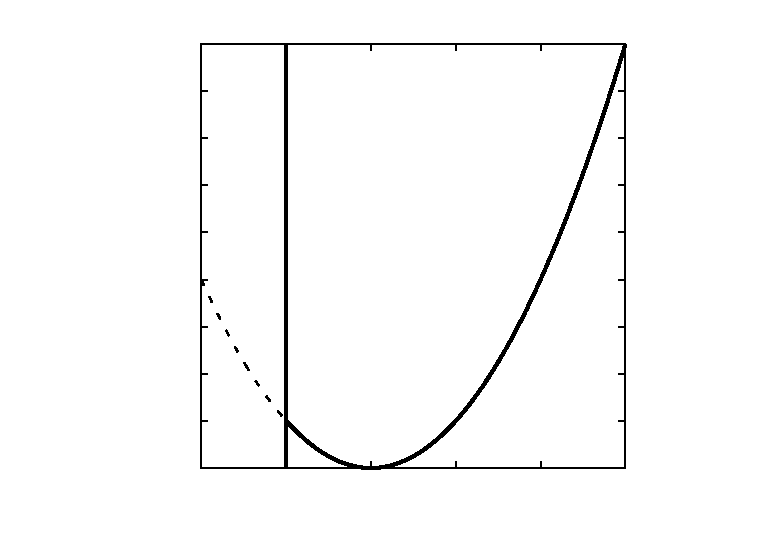
\includegraphics{delta_mass}}%
    \gplfronttext
  \end{picture}%
\endgroup

\caption{Scaling dimensions $\Delta$ corresponding to a given bulk mass for a scalar field, alongside the unitarity bound $\Delta\geq 1$.}
\end{figure}

This was for scalar fields. Higher-spin fields will be dual to operators of the same spin on the boundary and the $m-\Delta$ equation will be modified. For example, $(\frac{1}{2},\frac{1}{2})$ vectors will have

\begin{equation}
	R^2 m^2 = (\Delta-1)(\Delta-3)
	\label{}
\end{equation}

while $(1,1)$ symmetric tensor will instead have the same equation as scalars:

\begin{equation}
	R^2 m^2 = \Delta (\Delta-4)
	\label{}
\end{equation}

The relevance of this is that the operators coupled to massless spin $1$ or $2$ bosons must be conserved currents by gauge invariance, and so the operators dual to a massless bulk photon or graviton are a conserved vector current and the stress-energy tensor, respectively. The anomalous dimensions of these conserved currents must vanish, and indeed $\Delta_J = 3$ and $\Delta_T = 4$ are canonical.

\section{AdS/CFT over a cone}

As seen above, the original motivation for the AdS/CFT conjecture is the identification of a system of $N$ coincident D3-branes in a $\mathbb{R}^{1,9}$ Minkowski background and the corresponding 3-brane supergravity solution. In an appropriate low-energy limit a system of closed IIB strings on flat spacetime decouples in both pictures, suggesting it should be conjectured that the remaining parts are equivalent. These are respectively $\mathcal{N}=4$, $SU(N)$ SYM on $\mathbb{R}^{1,3}$ and IIB strings on $\ads 5 \times \mathbb{S}_5$.

We repeat this reasoning, but in the more interesting case where the background for the D3-branes is generalized as $\mathbb{R}^{1,3} \times X_6$, where $X_6$ is a cone over a base 5-manifold $Y_5$. Our intention is to build holographic dualities for the larger set of theories described in chapter \ref{chap:cones}. We anticipate the bulk dual in this case is IIB strings over $\ads 5 \times Y_5$.

In addition, we restrict to $X_6$ being Calabi-Yau, that is being K\"ahler with holonomy $\subset SU(3)$, because of the reasons detailed in section \ref{sec:generalcones}; equivalently, we only consider Sasaki-Einstein 5-folds for bases.% The complex structure on the cone induces a vector field on the base, the Reeb vector:%nota: da scholarpedia
%
%\begin{equation}
%	\xi := J (r \partial_r)
%\end{equation}
%
%where $J$ is the complex structure on the cone and $\xi$ is to be thought of as restricted to, say, ${r=1} \cong Y_5$; this is a Killing vector on the base, inducing a 1-dimensional foliation. The dual form, $\theta = g_{ij} \xi^i dx^j$, is a contact form for the base, contact meaning the 2-form on the cone
%
%\begin{equation}
%	\omega = t^2 d\theta + t dt \wedge \theta
%\end{equation}
%
%is symplectic. This is of course the symplectic form associated to the hermitian structure.\\

After placing 3-branes in this $\mathbb{R}^{1,3} \times X_6$ background, parallel to the Minkowski, the resulting geometry from their backreaction is:

\begin{equation}
ds^2 = H^{-1/2}(r,y) \, dx_\mu dx^\mu + H^{1/2}(r,y) \, ds_6^2
\end{equation}

Where $x^{0,\ldots,3}$ are coordinates parallel to the brane stack, $r$ is the radial coordinate and the remaining $y^{1,\ldots,5}$ parametrize the cone's base $Y_5$. This is a simple generalization of the flat-background 3-brane solution of \ref{sec:pbranes}, by substitution of $\mathbb{S}^5$ with $Y_5$. The above form can be argued for purely in terms of the $SO(1,3)$ symmetry acting on the $x^\mu$; the symmetry of the transverse dimensions is instead in general broken unless the branes lie exactly on the singularity, therefore the warp factor will depend also on $y^i$.

The equations of motion implies the function $H$ is harmonic $\nabla H(r) = 0$, identically to the flat-space case, since the branes are again extremal states.

If the branes are coincident and on the singularity, the corresponding harmonic potential is

\begin{align}
 H(r) = 1 + \frac{R^4}{r^4} && R^4 = 4 \pi g_s N \alpha'^2 
\end{align}

The near-horizon limit ($r\rightarrow 0$) in that case can be read immediately:

\begin{equation}
ds^2 = \frac{ dx_\mu dx^\mu + dz^2}{z^2} + ds_5^2
\end{equation}

where $z := 1/r$; this is evidently the product metric on $\ads 5 \times Y_5$.

Therefore, if it is possible to adapt the original argument for AdS/CFT for this situation, the existence a holographic duality can be established between the D3-brane worldvolume theory at the conical singularity and IIB strings (or, less ambitiously, supergravity) on $\ads 5 \times Y_5$.

On the quiver theory side, it was already seen how generalizing $\mathbb{S}^5 \rightarrow Y_5$ introduces novel features such as baryonic moduli and marginal deformations in addition to the coupling $\tau$.

%We note that the introduction of a conical singularity results in reduced supersymmetry. Unbroken SUSY generators are identified from the Killing spinor equation:
%
%\begin{equation}
%	\left(\partial_\mu + \frac{1}{4} \omega_{\mu\alpha\beta} \Gamma^{\alpha\beta} \right) \eta = 0
%\end{equation}
%
%Explicitly for the cone metric \ref{conemetric}:
%
%\begin{equation}
%	\left(\partial_i + \frac{1}{4} \omega_{ijk} \Gamma^{jk} + \frac{1}{2} \Gamma^r_i \right) \eta = 0
%\end{equation}
%
%this is, as expected, coincident with the ($Y_5$ sector of) Killing spinor equation for the backreacted $AdS_5 \times Y_5$ geometry, including also the effect of $F_5$. This is to show there is a match between the unbroken SUSYs in the bulk theory and in the boundary.\\
%
%If the cone is of holonomy $SU(n)$, this will result in a reduction of supersymmetries by a factor of $2^{1-n}$ with respect to $\mathbb{M}^{10}$ Minkowski. In particular, if $X_6$ is Calabi-Yau, then the $32 = 16 \times 2$ fermionic generators of IIB SUGRA are reduced to $32 \times 2^{-2} = 8$, which means the SCFT in $4D$ has $\mathcal{N}=1$ (in contrast to the usual SUSY algebra, the $\mathcal{N}=1$ $4D$ superconformal group has both $4$ supertranslations and $4$ additional fermionic superconformal generators). If, instead, we were to consider the more restrictive case of manifolds of $SU(2)$ holonomy, there would be $16$ unbroken supersymmetries signaling an $\mathcal{N}=2$ dual SCFT.
%
%%\section{The Klebanov-Witten model}
%%
%%\cmmnt{???}
%%
%%A well-known specific example of SCFT holographically dual to D-branes in a Calabi-Yau cone has been introduced in \cite{KW_SCFT}. In this case the base of the cone is the manifold $T^{1,1} = (SU(2)\times SU(2))/U(1)$, where $U(1) \subset SU(2)_L\times SU(2)_R$ is generated by $\sigma^3_L + \sigma^3_R$.\\
%%
%%We give a characterization of the cone $X_6$ over $T^{1,1}$ as a submanifold of $\mathbb{C}^4 \ni (A^1,A^2,B^1,B^2)$ given by
%%
%%\begin{equation}
%%	|A^1|^2 + |A^2|^2 - |B^3|^2 - |B^4|^2 = 0
%%\end{equation}
%%
%%quotiented by $U(1)$ acting on $A^i$ with charge $1$ and $B^i$ with charge $-1$. This makes the $SU(2)\times SU(2) \approx SO(4)$ symmetry manifest with the two copies of $SU(2)$ acting respectively only on $A^i$ and $B^i$.\\
%%
%%
%%The holographic dual theory to a stack of $N$ D3-brane moving in the background given by $\mathbb{R}^4$ times the cone over $T^{1,1}$ is found to be an $\mathcal{N}=1$ superconformal quiver gauge theory with gauge group $SU(N)\times SU(N)$, with chiral superfields $A^i$, $B^i$ ($i=1,2$) transforming respectively in the bifundamentals $(\mathbf{N},\mathbf{\bar N})$, $(\mathbf{\bar N},\mathbf{N})$. The $SU(2)\times SU(2)$ isometry in the bulk is here implemented as a "flavour" global symmetry acting separately on $A^i$ and $B^i$. Moreover, the diagonal $U(1)$ reappears as a baryonic symmetry where again $A^i$ has charge $1$ and $B^i$ charge $-1$.\\
%%
%%
%%\cmmnt{relazione fra i campi della CFT e la posizione delle D-brane, moduli space mesonico e totale, un po' di più sul KW}
%%


\chapter{Holographic effective field theories}


\cmmnt{definizione di HEFT come in \cite{MZ}}

\section{Bulk moduli}

\cmmnt{identificazione dei moduli del bulk: numeri di Betti e condizioni globali sui potenziali, moduli della struttura K\"ahler}

We now identify the moduli of the bulk string theory. This will include deformations of the background metric and of the RR potentials, parametrized by particular types of $k$-forms. Therefore, a great deal of information about them can be obtained just from examining the topology of the cone $X_6$.\\

First of all, we take as an assumption that the third Betti number of the cone vanishes:

\begin{equation}
	b_3(X) = 0 \label{bettiX3}
\end{equation}

It can be proven from Myers' theorem that $Y_5$ being Sasaki-Einstein means the following Betti numbers vanish:

\begin{equation}
	b_1(Y) = b_4(Y) = 0 \label{bettiY14}
\end{equation}

It's also possible to prove that

\begin{equation}
	b_1(X) = b_5(X) = b_6(X) = 0
\end{equation}

The vanishing of the odd Betti numbers for $X_6$ means $Dp$-branes with $p = 1,3,5$ cannot be wrapped around nontrivial $p$-cycles.\\

We recall the long sequence involving relative homology groups:

\begin{equation}
	\ldots \rightarrow H^{i-1}(Y) \rightarrow H^{i}(X,Y) \rightarrow H^i(X) \rightarrow H^i(Y) \rightarrow H^{i+1}(X,Y) \rightarrow \ldots
\end{equation}

where $H^i(X,Y;\mathbb{R})$ is the relative homology group - closed $k$-forms on $X$ vanishing on $Y$ modulo exact forms with the same property - and when the $;\mathbb{R}$ is omitted we implicitly mean the base field is $\mathbb{R}$. We cut the sequence short by setting $i=2$ and noting $H^1(Y) = 0$ as of \ref{bettiY14} and $H^3(X,Y) \subset H^3(X) = 0$ as of \ref{bettiX3}; the short exact sequence is

\begin{equation}
	0 \rightarrow H^2(X,Y) \rightarrow H^2(X) \rightarrow H^2(Y) \rightarrow 0
\end{equation}

Implying $H^2(X) = H^2(Y) \oplus H^2(X,Y)$. Applying Poincaré duality on the two components and counting dimensions gives

\begin{equation}
	b_2(X) = b_3(Y) + b_4(X)
\end{equation}

This result will be useful in parametrizing deformations of the axio-dilaton $\tau$ and the 2-forms $C_2$ and $B_2$. In particular, combining these fields into a single complex $2$-form $C_2 - \tau B_2$, for any given value of $\tau$ the deformations of this form are decomposable in $b_2(X)$ complex parameters, to which we then append one additional parameter for deformations of $\tau$. Making use of the above splitting, these are divided in $b_3(Y) + 1$ 'boundary' complex parameters counting non-dynamical deformations, and $b_4(X)$ 'bulk' dynamical complex moduli.\\

\cmmnt{$C_4$ moduli}

Having dealt with RR moduli, we now consider the moduli of the K\"ahler structure of the background. Since $b_3(X) = 0$ by hypothesis, the complex structure is rigid. There are instead moduli for the K\"ahler form $J$; in particular we know from \cmmnt{citazione teoremi esistenza} that every cohomology class $[J]$ of $H^2(X)$ contains a single representative Ricci-flat K\"ahler form $J$, so that $H^2(X)$ is the moduli space for the K\"ahler structure. We can expand the cohomology class as

\begin{equation}
	[J] = v^a [\omega_a] \label{integraldecomposition}
\end{equation}

with $[\omega_a]$ being a basis for the integral cohomology $H^2(X;\mathbb Z)$, as the latter modulo torsion is a lattice sitting in $H^2(X;\mathbb R)$. This means

\begin{equation}
	\delta [J] = \delta v^a [\omega_a]
\end{equation}

meaning there exist representatives in the classes such that the equation without square brackets holds. Since small variations of the K\"ahler form must be $(1,1)$ harmonic forms \cmmnt{reference}, we then know there exist $(1,1)$ harmonic representatives $\omega_a$ for the aforementioned basis of classes. Returning to \ref{integraldecomposition} we can rewrite it as

\begin{equation}
	J - v^a \omega_a \in [0]
\end{equation}

But for the LHS to belong to the zero class just means to be exact. Therefore

\begin{equation}
	J = J_0 + v^a \omega_a \label{JandJ0}
\end{equation}

with $J_0$ being exact and $(1,1)$. Note the linearity of this parametrization is an illusion of notation: the condition $\Delta \omega_a = 0$ depends on the metric and so on both $J_0$ and $v^a$.


\section{Boundary moduli}

\cmmnt{descrizione della CFT holografica tipica (quiver), di nuovo classificazione dei moduli}

\section{Effective action}

\cmmnt{azione efficace calcolata in \cite{MZ}; forse anche la derivazione?}

\section{The Klebanov Witten HEFT}

\cmmnt{Calcolo esplicito della HEFT per il KW}


\chapter{The $Y^{(2,0)}$ HEFT}

%We now finally tackle the explicit determination of the Lagrangian of the effective field theory describing the low-energy dynamics of the $Y^{2,0}$ field theory described in \ref{sec:squares}, through techniques introduced in \cite{MZ}.

\section{K\"ahler moduli}

The general Calabi-Yau deformation of the $Y^{2,0}$ cone is already well-known (\cmmnt{refs}) in real coordinates as:

\begin{equation}
ds^2 = \kappa^{-1}(r)dr^2 + \frac{1}{9} \kappa(r) r^2 (d\psi + \cos\theta_L d\phi_L + \cos\theta_R d\phi_R)^2 + \frac{1}{6} r^2 d\Omega_L^2 + \frac{1}{6}(r^2+a^2) d\Omega_R^2 \label{y20metric} \end{equation}
\begin{equation}
	\kappa(r) = \frac{1 + \frac{9a^2}{r^2} - \frac{b^6}{r^6}}{1+ \frac{6a^2}{r^2}}
\end{equation}

with $a,b$ the two unique real moduli. The topology is that of an $\mathbb{R}^2$ bundle over $\mathbb{S}^2 \times \mathbb{S}^2$.\\

For the purpose of building the effective theory, however, this metric must be rewritten in a complex chart. To that end, we try to find the general CY metric on a $\mathbb{C} \rightarrow \mathbb{CP}^1 \times \mathbb{CP}^1$ bundle; on the spheres of the base we take the round metric, given by the K\"ahler forms $j^L$ and $j^R$. It's easy to verify explicitly that, given any set of complex coordinates on the base $(y_L,y_R)$,

\begin{equation}
	j^L \wedge j^R = e^{-\Lambda k} dy^L \wedge dy^R \wedge d\bar y^L \wedge d\bar y^R
\end{equation}

with $k = k^L + k^R$ the total base potential, and for some $\Lambda$ depending on the overall size of the spheres (for unit radius, $\Lambda = 1$).\\

We also introduce the function $t$ of the fibral coordinate $\zeta$ as 

\begin{equation}
	t = |\zeta|^2 e^{\Lambda k}
\end{equation}

We then start from the following ansatz for the K\"ahler potential:

\begin{equation}
	k_X = f(t) + \alpha k^L + \tilde\alpha k^R
\end{equation}

where $\alpha,\tilde\alpha$, controlling the volume at $t=0$ of the base 2-spheres, parametrize the Ricci-flat K\"ahler resolutions of the cone. We are now set to prove that there is always an $f(t;\alpha,\tilde\alpha)$ that makes the metric Ricci-flat.\\

The corresponding K\"ahler form is straightforward:

\begin{equation}
	J = A^L j^L + A^R j^R + i e^{\Lambda k} (f' + t f'') (d\zeta + \Lambda \zeta \partial k) \wedge (\mathrm{c.c.})
\end{equation}

\newcommand{\fibral}{e^3 \wedge \bar e^{\bar 3}}

with $A^L = \alpha + \Lambda t f'(t)$ and  $A^R = \tilde\alpha + \Lambda t f'(t)$. This is more simply $J = J_M + M \fibral$, where $J_M$ is the purely basal part, $e^3 = d\zeta + \Lambda \zeta \partial k$ and $M$ is a scalar factor. The volume form is then clearly

\begin{equation}
	J \wedge J \wedge J = 3 A^L A^R M \, j^1 \wedge j^2 \wedge \fibral
\end{equation}

as all other terms in the cube vanish. Since the volume form is $\sqrt{\det g} \, d\Omega \wedge \bar \Omega$, with $\Omega = d\zeta \wedge dy^L \wedge dy^R$, and the Ricci tensor for a K\"ahler space is proportional to $\partial \bar \partial \ln \det g$, then the condition for Ricci-flatness is equivalent to the prefactor of $\Omega \wedge \bar \Omega$ in $J\wedge J \wedge J$ being constant, that is to say

\begin{equation}
	(\alpha + \Lambda t f')(\tilde{\alpha} + \Lambda t f') \frac{d}{dt} (\Lambda t f') = c \label{rflatcondition}
\end{equation}

or, having defined $y = \Lambda t f'$,

\begin{equation}
	(\alpha + y)(\tilde{\alpha} + y) y' = c
\end{equation}

Since $f(t)$ must be regular as $t=0$, and $f' = \frac{y}{\Lambda t}$, it must be that $y$ goes to zero at least as fast as $t$ as $t\rightarrow 0$; this condition eliminates the freedom from the constant of integration for equation \ref{rflatcondition}. The constant $c$ on the other hand can be readily reabsorbed into a $t$ rescaling. Therefore there should be a unique $y$ (and so a unique $f$ up to unconsequential constant shifts) that gives a Ricci-flat metric. Let us see this explicitly: we integrate \ref{rflatcondition} to obtain

\begin{equation}
	\frac{y^3}{3} + \frac{\alpha + \tilde{\alpha}}{2} y^2 + \alpha \tilde{\alpha} y = ct + d \label{rflatintegrated}
\end{equation}

And then the regularity condition $y(0)=0$ is satisfied with $d=0$, and this cubic equation for $y$ is immediately seen to have one single real solution for any positive values of $\alpha^i$, $c$.\\

Before exhibiting the explicit form of $y(t;\alpha,\tilde\alpha)$, let us express the K\"ahler form in terms of $y$ and show it's actually equal to the real-coordinate metric \ref{y20metric}. We have

\begin{align}
	\label{Jintermsofy}
	J & =  (\alpha + y) j^1 + (\tilde{\alpha} + y) j^2 + \frac{ie^{\Lambda k}}\Lambda y' \fibral\\
	  & =  (\alpha + y) j^1 + (\tilde{\alpha} + y) j^2 + \frac{ie^{\Lambda k} \,c}{\Lambda (\alpha + y)(\tilde{\alpha} + y)} \fibral
\end{align}

Now, we parametrize the fiber as $\zeta = e^{-\Lambda k/2} t^{1/2} e^{i\psi}$, and the 2-spheres with spherical coordinates $\theta_i$, $\phi_i$ which fixes $\Lambda = 1$. Then the metric corresponding to $J$ is

\begin{equation}
	ds^2 = A^L d\Omega^2_L + A^R d\Omega^2_R + \frac{y'}{t} \left( \frac{dt^2}{4} + t^2 (d\psi + \sigma)^2 \right)
\end{equation}

Where $\sigma = -i\frac{\Lambda}{2}(\partial k - \bar \partial k)$. But the $t-\psi$ part is simply

\begin{equation}
	ds^2 = \frac{1}{4y't} dy^2 + (y' t) (d\psi + \sigma)^2
\end{equation}

Exploiting both \ref{rflatcondition} and its integrated form \ref{rflatintegrated} we rewrite

\begin{align}
	y't & = \frac{1}{A^L A^R} \left( \frac{y^3}{3} + \frac{\alpha + \tilde{\alpha}}{2} y^2 + \alpha \tilde{\alpha} y \right)\\
	& = 3cr^2 \frac{1+ \frac{3}{2} \frac{\tilde{\alpha} - \alpha}{r^2} + \frac{\alpha^{2}(\alpha - 3 \tilde{\alpha})}{2r^6} }{1+ \frac{\tilde{\alpha} -\alpha}{r^2} }\\
	& = 3cr^2 \kappa(r)
\end{align}

provided we make the identifications

\begin{align}
	a^2 = \frac{1}{6}(\tilde{\alpha} - \alpha) && b^6 = \frac{\alpha^{2}(3\tilde{\alpha}-\alpha)}2
	\label{<++>}
\end{align}

The final coordinate change to the $r$ coordinate is then given by $r^2 = A^L = y + \alpha$ - note this renders the inherent symmetry between the left and right 2-cycles non-manifest. The resulting metric, after taking $c=1/3$, is precisely \ref{y20metric}. Thus, as the latter is the most general Calabi-Yau deformation of the $Y^{2,0}$ cone, we have to conclude that the two-parameter family of metrics \ref{Jintermsofy} in complex coordinates coincides with it.\\

Now we're left with solving for the explicit form of $y$. Switching temporarily to $z = y + (\alpha + \tilde\alpha)/2$ equation \ref{rflatintegrated} is brought into depressed form:

\begin{equation}
	z^3 - \frac{3}4 (\alpha - \tilde\alpha)^2 = ct + D
	\label{depressed}
\end{equation}

Where

\begin{equation}
	D = \frac{1}{12}(-\alpha^3 + 3 \alpha^2 \tilde\alpha + 3 \alpha\tilde{\alpha} - \tilde{\alpha}^3) = \frac{b^6-36a^6}{3}
	\label{dprime}
\end{equation}

So that the explicit solution for $y$ is

\begin{equation}
	z = |\alpha - \tilde \alpha| C_{1/3} \left( 12 \frac{ct + D}{|\alpha-\tilde\alpha|^3} \right) 
	\label{explicitz}
\end{equation}
\begin{equation}
	y = z - \frac{\alpha + \tilde{\alpha}}2
	\label{explicitY}
\end{equation}

where we defined the function $C_{1/3} = \ch(1/3 \; \ch^{-1}(x))$; that \ref{explicitY} solves \ref{depressed} can be readily verified by means of the trigonometric identity $\ch(3x) = 4 \ch^3(x) - 3 \ch(x)$.\\

Fixing $c=1/3$ for future convenience and introducing the notation $\delta = \alpha - \tilde{\alpha}$, $\sigma = \alpha + \tilde{\alpha}$, the K\"ahler form is explicitly given by

\begin{equation}
	J(\sigma,\delta) = \left(  z + \frac{\delta}{2}\right) j^1 + \left(z-\frac{\delta}{2}\right) j^2 + ie^k z' e^3 \wedge \bar e^{\bar 3}
	\label{}
\end{equation}

\begin{equation}
	z(t;\sigma,\delta) = \delta \;C_{1/3} \left( \delta^{-3} \left( 4t + \frac{\sigma(3\delta^2 - \sigma^2)}{2} \right) \right)
	\label{}
\end{equation}

~\\\cmmnt{e qua si copincollerà il resto delle note quanto saranno definitive}\\




%        File: notes.tex
%     Created: mar ago 23 10:00  2016 C
% Last Change: mar ago 23 10:00  2016 C
%
%\documentclass[a4paper]{article}
%\usepackage{amssymb}
%\usepackage[]{amsmath}
%\usepackage[]{hyperref}
%
%\usepackage[]{graphicx}
%
\graphicspath{{images/}}
%\usepackage{color}
%
%\DeclareMathOperator{\ch}{ch}

\label{chap:y20}

%\setlength{\parindent}{0cm}
%i
%\begin{document}

Having secured the tools required, we are now ready to take on the holographic effective theory of the $Y^{2,0}$ theory introduced in \ref{sec:squares}, to which this thesis is dedicated, and whose low-energy effective dynamics had not been investigated so far.

Exploiting the architecture established in the previous chapter, we will identify the fields and parameters on the gravitational dual which enter in the low-energy description, and determine the exact form of the effective action for this strongly-coupled, minimally supersymmetric gauge theory. 

The bulk of this calculation turns out to be occupied by the determination of the Ricci-flat metric of the general Calabi-Yau deformation of the $X^{2,0}$ cone over the Sasaki-Einstein base $Y^{2,0}$; the deformations are in this case parametrized by two moduli, measuring the volumes of a 2-cycle and a 4-cycle respectively. Due to the introduction of this 4-cycle blowup (ultimately arising from the $\mathbb{Z}_2$ orbifold) the metric is quite more complicated than the deformation of the conifold, which only featured a 2-cycle blowup. As part of our original contributions we will thus present therefore our determination of the deformed metric in complex coordinates for generic values of the two moduli.

\section{General properties}

The features of the SCFT analyzed in \ref{sec:squares} can be rederived holographically. First of all, the homology of the singular cone will allow for the counting of supergravity moduli and marginal deformations that can be seen to match with those found from the field theory side. We recall the metric on the $X^{2,0}$ cone is

\begin{equation}
	ds_6^2 = dr^2 + r^2 ds_5^2
	\label{}
\end{equation}
\begin{equation}
	ds_5^2 = \frac{1}{9}\left( d\psi + \sum_{i=1,2} \cos\theta_i d\phi_i\right)^2 + 
	\frac{1}{6} \sum_{i=1,2} \left(d\theta_i^2 + \cos^2\theta_i d\phi_i^2 \right)
\end{equation}
\begin{equation}
	\psi \in [0,2\pi]
	\label{}
\end{equation}

Since the conifold base had topology $\mathbb{S}^2 \times \mathbb{S}^3$\cite{Candelas}, this base will be $Y^{2,0} \cong (\mathbb{S}^2 \times \mathbb{S}^3)/\mathbb{Z}_2$. The new Betti numbers of the cone are easily read from the fact that the generic deformation of $X^{2,0}$ is a bundle $\C \rightarrow \cpone \times \cpone$, which we will prove in the next section. First, we have $b_3(Y^{2,0}) = b_3(\ess^2 \times \ess^3) = 1$, while $b_4(X^{2,0}) = b_4(\cpone \times \cpone) = 1$. Finally, using \eqref{bettidentity}, $b_2(X_6) = 2$. To summarize:

\begin{equation}
	b_2(X_6) = 2,\quad b_4(X_6) = 1,\quad b_3(Y_5) = 1\,.
	\label{}
\end{equation}


According to the discussion of section \ref{sec:heftkm}, there will be $b_2(X) = 2$ independent harmonic forms $\omega_a$ from the two 2-cohomology classes, and these will parametrize deformations of the K\"ahler form:

\begin{equation}
	J = J_0 + v^a \omega_a\,,
	\label{}
\end{equation}

with two associated moduli $v^a$. These forms will be divided in $b_3(Y) = 1$ ``non-compact'' form $\tilde\omega$, and $b_4(X) = 1$ ``compact'' form $\hat \omega$. The latter, associated with the blow-up of the 4-cycle, is the novel feature with respect to the Klebanov-Witten model, which only featured $\tilde\omega$.

In addition, $\omega_a$ will generate $A_2 - \tau B_2$ deformations:

\begin{equation}
	(A_2 - \tau B_2) = l_s^2 \left( \beta \, \hat \omega + \lambda \, \tilde \omega \right) \,.
	\label{}
\end{equation}

However, only the renormalizable deformation will yield a dynamical field $\beta$, as shown in section \ref{sec:hefttwo}. The parameter $\lambda$ will be a marginal parameter, alongside the axio-dilaton $\tau$.

Once the $v^a = (\hat v, \tilde v)$ K\"ahler moduli have been transformed into the $\rho^a = (\hat \rho, \tilde \rho)$ fields according to \eqref{rhov}, it is now possible to match the counting of moduli and marginal parameters between the bulk and the $Y^{2,0}$ CFT as following:

\begin{center}
\begin{tabular}{ccc}
	 		& $\ads 5 \times Y_5$ & CFT \\ \midrule \midrule
			& $ z_I^i$ & $3N$ mesons\\ \cmidrule{2-3} 
dynamic 		& $\hat \rho$ & \multirow{3}{*}{$\chi-1 = 3$ baryons} \\
moduli			& $\tilde \rho$ & \\
			& $ \beta$ & \\ \midrule
marginal	& $\tau$ 	&  \multirow{2}{*}{$2$ marginal deformations}	\\
parameters			& $\lambda$ &	
\end{tabular}
\end{center}

Since the dynamical fields of the effective theory have been identified and matched, the explicit construction of the $\omega_a$ forms will allow for the specification of their dynamics. In practice, this requires determining the metric in complex coordinates of the general Calabi-Yau deformation of the $X^{2,0}$ cone. This metric is known in real, ``polar'' coordinates (see \eqref{genCYy20cones}) but a diffeomorphism to a chart compatible with the K\"ahler structure is not. In the next section, we present our solution to this problem in the form of an explicit expression for the Calabi-Yau metric in a set of complex coordinates, and verify the match with the known real parametrization.


\section{K\"ahler form}

The metric of the general Calabi-Yau deformation of the $X^{2,0}$ cone is already well-known in real coordinates as (repeating \eqref{genCYy20cones})

\begin{align}
\begin{split}
ds^2 \,= \;\, &\kappa^{-1}(r)\,dr^2 \;+\; \frac{1}{9} \kappa(r) r^2 \large(d\psi + \cos\theta_L d\phi_L + \cos\theta_R d\phi_R\large)^2\\
& + \frac{1}{6} r^2 d\Omega_L^2 \,+ \, \frac{1}{6}(r^2+a^2) d\Omega_R^2\,, \label{y20metric} 
\end{split}
\end{align}

\begin{equation}
	\kappa(r) = \cfrac{1 + \cfrac{9a^2}{r^2} - \cfrac{b^6}{r^6}}{1+ \cfrac{6a^2}{r^2}}\,,
\end{equation}

with $a,b$ the two unique real moduli. The topology is that of an $\mathbb{R}^2$ bundle over $\mathbb{S}^2 \times \mathbb{S}^2$. We take it as an assumption that this matches with the complex structure associated to the K\"ahler form so that this is the total space of a $\mathbb{C}$ bundle over $\mathbb{CP}^1 \times \mathbb{CP}^1$ - we will confirm this a posteriori when we'll provide the complex-coordinates expression and show it agrees with the real form.

With this assumption, we search for the general CY metric on a $\mathbb{C} \rightarrow \mathbb{CP}^1 \times \mathbb{CP}^1$ bundle; on the spheres of the base we take the round metric, given by the K\"ahler forms $j^L$ and $j^R$ generated by K\"ahler potentials\footnote{Attention should be paid to the fact that the potentials are different for different coordinates.} $k^L$, $k^R$. We thus, having chosen any local complex charts $y_L$, $y_R$ on the two basal spheres (e.g.: stereographic) and a fibral coordinate $\zeta$, have a local chart $z^i = (\zeta,y_L,y_R)$ for the bundle. It is easy to verify explicitly that, given any set of complex coordinates on the base $(y_L,y_R)$,

\begin{equation}\label{spheresareEinstein}
	j^L \wedge j^R = e^{-\lamkah}\, \left(dy^L \wedge dy^R \wedge d\bar y^L \wedge d\bar y^R\right)\,,
\end{equation}

for some $\Lambda$ depending on the overall size of the spheres (for the unit sphere, $\Lambda = 1$).

We also introduce the radial coordinate $t(\zeta,y_L,y_R)$ as 

\begin{equation}
	t := |\zeta|^2 e^{\Lambda k}\,.
\end{equation}

We then propose the following ansatz for the K\"ahler potential of the resolved cone:

\begin{equation}
	k_0 = f(t) + \alpha k^L + \tilde\alpha k^R \label{y20potentialansatz}
\end{equation}

where the moduli $\alpha,\tilde\alpha$, controlling the volume at $t=0$ of the base 2-spheres, should parametrize the Ricci-flat K\"ahler resolutions of the cone. We now prove that there is always an $f(t;\alpha,\tilde\alpha)$ that makes the metric Ricci-flat.

The K\"ahler form generated by \eqref{y20potentialansatz} is straightforward:

\begin{align}
	\begin{split}\label{y20kahlerformansatz}
	J &= \, \AL j^L + \, \AR j^R \\&+ i e^{\lamkah} (f' + t f'') \, (d\zeta + \Lambda \zeta \partial k) \wedge (\mathrm{c.c.})
\end{split}
\end{align}

\newcommand{\fibral}{e^3 \wedge \bar e^{\bar 3}}

%with $A^L := \alpha + \Lambda t f'(t)$ and  $A^R := \tilde\alpha + \Lambda t f'(t)$. 

%This is more simply expressed as

%\begin{equation}
%J = J_M + M \fibral\,,
%\end{equation}

%where $J_M$ is the purely basal part, $e^3 = d\zeta + \Lambda \zeta \partial k$ and $M:= ie^{\Lambda k} \left( f' + t f'' \right)$ is a scalar factor. The volume form is then
The form $J = J_{\ibj}\, dz^i \wedge d\bar z^{\bar\jmath}$ defines a metric $ds^2 = J_{\ibj}\, dz^i \otimes d\bar z^{\bar\jmath}$, or equivalently $g_{\ibj} = J_{\ibj}\,$. We would like to identify the condition on $f(t)$ for such a metric to be Ricci-flat. In a K\"ahler manifold, and in a given local chart, the Ricci form is given by\cmmnt{ref}

\begin{equation}
	R = i \partial \bar\partial \log \sqrt{ \det g}\,,
	\label{}
\end{equation}

so that Ricci-flatness, $R = 0$, means $\det g = \det {J_{\ibj}}$ is a constant. However, note the volume form induced by the metric would be

\begin{equation}
	d\vol_{X_6} = \sqrt{\det g}\, \left(\Omega \wedge \overline \Omega\right)
	\label{volumeintermsofmetric}
\end{equation}

with $\Omega = d\zeta \wedge dy^L \wedge dy^R$ the holomorphic three-form on $X_6$. However, for a K\"ahler $3$-fold one has the equivalent expression in terms of the K\"ahler form:

\begin{equation}
	3! \, d\vol_{X_6} = J\wedge J \wedge J 	\label{}
\end{equation}

Having defined $e^3 := d\zeta + \Lambda \zeta \partial (\kah)$, this is

\begin{equation}
	= 3 \AL \AR i e^{\lamkah} \left(f'+tf''\right) \left(j^1 \wedge j^2 \wedge \fibral \right)\,
	\label{}
\end{equation}

and using \eqref{spheresareEinstein}:

\begin{equation}
	= (\AL)(\AR) \left( f' +tf'' \right) \Omega \wedge \overline \Omega
	\label{volumeintermsofkahler}
\end{equation}

By comparing \eqref{volumeintermsofkahler} with expression \eqref{volumeintermsofmetric} for the volume form, we have to deduce that Ricci-flatness is equivalent to the following expression being constant:

%as all other terms in the cube vanish. Since the volume form is also $\sqrt{\det g} \, d\Omega \wedge \overline \Omega$, with $\Omega = d\zeta \wedge dy^L \wedge dy^R$ the holomorphic three-form, and the Ricci tensor for a K\"ahler space is proportional to $\partial \bar \partial \ln \det g$, then the condition for Ricci-flatness is equivalent to the prefactor of $\Omega \wedge \bar \Omega$ in $J\wedge J \wedge J$ being constant, that is to say

\begin{equation}
	(\alpha + \Lambda t f')(\tildd{\alpha} + \Lambda t f') \frac{d}{dt} (\Lambda t f') =: c 
\end{equation}

or, having defined $y(t) := \Lambda t f'(t)$,

\begin{equation}
	(\alpha + y)\,(\tildd{\alpha} + y)\, y' = c\,. \label{rflatcondition}
\end{equation}

This differential equation (second order in $f(t)$) is thus the condition for the metric resulting from the ansatz \eqref{y20potentialansatz} to be Ricci-flat, and therefore a supergravity solution.

Since $f(t)$ must be regular as $t=0$, and $f' = \frac{y}{\Lambda t}$, it must be that $y$ goes to zero at least as fast as $t$ as $t\rightarrow 0$; this condition eliminates the freedom from the constant of integration for equation \eqref{rflatcondition}. The constant $c$ on the other hand can be readily reabsorbed into a $t$ rescaling. Therefore there should be a unique $y$ (and so a unique $f$ up to unconsequential constant shifts) that gives a Ricci-flat metric. In appendix \ref{appendix:solutioncubic} we prove that the solution is indeed unique, and the solution to \eqref{rflatcondition} is given by


\begin{equation}
	y(t;\alpha,\tildd\alpha)  = |\alpha - \tildd\alpha| \Cfun { 12 \frac{ct + D}{|\alpha-\tildd\alpha|^3} } - \frac{\alpha + \tildd\alpha}{2}\,,
	\label{}
\end{equation}
\begin{equation}
	 D := \frac{1}{12}(-\alpha^3 + 3 \alpha^2 \tilde\alpha + 3 \alpha\tilde{\alpha} - \tilde{\alpha}^3) \,.
	\label{}
\end{equation}

While essential for our derivation of the HEFT, the explicit form above of $y(t;\alpha,\tilde\alpha)$ is not necessary to verify this metric matches with the real-coordinate form \eqref{y20metric}: let us express the K\"ahler form in terms of $y$ and show it actually coincides with the latter. We have

\begin{align}
	\label{Jintermsofy}
	J & =  (\alpha + y) j^1 + (\tilde{\alpha} + y) j^2 + \frac{ie^{\Lambda k}}\Lambda y' \fibral\\
	  & =  (\alpha + y) j^1 + (\tilde{\alpha} + y) j^2 + \frac{ie^{\Lambda k} \,c}{\Lambda (\alpha + y)(\tilde{\alpha} + y)} \fibral
\end{align}

Now, we parametrize the fiber as 

\begin{equation}
	\zeta = e^{-\Lambda k/2}\, \sqrt{t} \,e^{i\psi}\,,
\end{equation}

and the 2-spheres with spherical coordinates $\theta_i$, $\phi_i$ which fixes $\Lambda = 1$. Then the metric corresponding to $J$ is

\begin{equation}
	ds^2 = (\alpha+y)\, d\Omega^2_L + (\tildd\alpha + y) \,d\Omega^2_R + \frac{y'}{t} \left( \frac{dt^2}{4} + t^2 (d\psi + \sigma)^2 \right)
\end{equation}

Where $\sigma := -i\frac{\Lambda}{2}(\partial k - \bar \partial k) = \sum_i \cos\theta_i d\phi_i$. But the $t-\psi$ part is simply

\begin{equation}
	ds^2 = \frac{1}{4y't} dy^2 + (y' t) (d\psi + \sigma)^2
\end{equation}

Exploiting both the Ricci-flatness condition \eqref{rflatcondition} and its integrated form \eqref{rflatintegrated} we rewrite the expression $y't$ as

\begin{align}
	y'\,t & = \left(\frac{1}{(\alpha + y)(\tilde\alpha + y)}\right) \left( \frac{y^3}{3} + \frac{\alpha + \tilde{\alpha}}{2} y^2 + \alpha \tilde{\alpha} y \right)\\
	& = 3c\,r^2 \left(
	{1+ \frac{3}{2} \frac{\tilde{\alpha} - \alpha}{r^2} + {\alpha^{2}(\alpha - 3 \tilde{\alpha})}{2r^6} }
	\right)\bigg/\left({1+ \frac{\tilde{\alpha} -\alpha}{r^2} }\right)\\
	& = 3c\,r^2 \left({1+\frac{9a^2}{r^2} - \frac{b^6}{r^6}}\right)\bigg/\left({1 + \frac{6a^2}{r^2}}\right) \\
	& = 3c\,r^2 \kappa(r)
\end{align}

provided we make the identifications

\begin{align}
	a^2 = \frac{1}{6}(\tilde{\alpha} - \alpha) && b^6 = \frac{\alpha^{2}(3\tilde{\alpha}-\alpha)}2
	\label{}
\end{align}

The final coordinate change to the (asymptotically) conical $r$ coordinate is then given by $r^2 := y + \alpha$ - note this renders the inherent symmetry between the left and right 2-cycles non-manifest\footnote{Clearly, we could swap $\alpha$ and $\tilde{\alpha}$ in all of the above definitions, with no consequence.}. The resulting metric, after taking $c=1/3$, is precisely the known real-coordinate metric \eqref{y20metric}. Thus, as the latter is the most general Calabi-Yau deformation of the $X^{2,0}$ cone, we have to conclude that the two-parameter family of metrics \eqref{Jintermsofy} in complex coordinates coincides with it.

Using the freedom to scale $t$ to fix $c=1/3$ for future convenience and introducing the notation 

\begin{equation}\label{convenientmoduli}
	\delta := \alpha - \tilde{\alpha}\,,\quad \sigma := \alpha + \tilde{\alpha}\,,
\end{equation}

the K\"ahler form is explicitly given by

\begin{equation}
	J(\sigma,\delta) = \left(  z + \frac{\delta}{2}\right) j^1 + \left(z-\frac{\delta}{2}\right) j^2 + ie^k z' e^3 \wedge \bar e^{\bar 3}\,
	\label{}
\end{equation}

\begin{equation}
	z(t;\sigma,\delta) = \delta \;\Cfun { \delta^{-3} \left( 4t + \frac{\sigma(3\delta^2 - \sigma^2)}{2} \right) }\,.
	\label{}
\end{equation}

Or, equivalently, in terms of the $y$ function:

\begin{equation}
	J(\sigma,\delta) = (y+\alpha) j^1 + (y+\tilde{\alpha})j^2 + ie^k y' e^3 \wedge \bar e^{\bar 3}
	\label{}
\end{equation}

Unfortunately, a closed-form expression for the K\"ahler potential seems impossible. The function $f(t)$ can nevertheless be written in integral form, as such:

\begin{equation}
	f(t;\sigma,\delta) = \int_0^{t} d\ln t' y(t')
	\label{}
\end{equation}

\section{K\"ahler moduli}

As we have seen, a very convenient basis of moduli for the K\"ahler structure is given by the sum and difference $\sigma$ and $\delta$ of the volume of the base spheres defined in \eqref{convenientmoduli}, up to a normalization which we will shortly determine. These correspond respectively to blowing up the two basal 2-cycles (which equates to a blowup of the product 4-cycle of the base) and to an antisymmetric blowing and shrinking of the two $\ess^2$ (a blowup of the difference 2-cycle). We'll examine this geometric structure in more detail in this section.

We will construct the two harmonic forms $\hatt\omega$ and $\tildd\omega$ by differentiating $J$ directly with respect to the relevant moduli, since (see \eqref{JandJ0})

\begin{equation}
	J = J_0 \,+ \, \hatt v \,\hatt \omega + \tildd v \,\tildd \omega
	\label{}
\end{equation}

A basis $(\hatt\omega,\tildd\omega)$ of harmonic two-forms will allow us to also parametrize deformations of the $A_2$ and $B_2$ fields according to \eqref{ABvariation}.

%As an aside, we check all forms obtained in this way from $J$ are primitive: in the $dy^1$, $dy^2$, $e^3$ basis the Kahler form is $\mathrm{diag}(A^L j^1_{1\bar 1}, A^R j^2_{2\bar 2}, i e^k y')$ so the contraction of $J$ with any derivative $\partial_x J$ of it with respect to a parameter is

%\begin{align}
%\begin{split}
%	J^{a\bar b}\partial_x J_{a\bar b} = \mathrm{Tr}\left( (J_{a\bar b})^{-1} \partial_x J_{a\bar b} \right) = A^{-1} \partial_x A + \tilde A^{-1} \partial_x \tilde A + (y')^{-1} \partial_x y' \\= \partial_x \ln \left( A \tilde A y' \right)	
%	\label{}
%\end{split}\end{align}
%
%which vanishes thanks to the Ricci-flatness equation.

As it is clear from our general discussion, we expect to be able to choose $(\hatt\omega,\tildd\omega)$ such that $\hatt\omega$ is normalizable in the sense of \eqref{defM} - this would be the form generating the blowup of the 4-cycle. The other form $\tildd\omega$ will be non-renormalizable and will correspond to a 2-cycle blowup, the same that was already present in the Klebanov-Witten theory. It is easy to see that the modulus $\hatt v$ relative to $\hatt \omega$ must be proportional to the sum $\sigma$ of the basal volumes, since the corresponding harmonic form $\frac{\partial J}{\partial \sigma}$ is normalizable. To show this, we consider the asymptotic behaviour of the K\"ahler form as $t\rightarrow \infty$. Defined

\begin{equation}
	T := \left( 4t + \frac{\sigma(3\delta^2 - \sigma^2)}{2} \right)
	\label{}
\end{equation}

we have

\begin{align}
	z \sim T^{1/3} && z' \sim T^{-2/3}\\	
	\frac{\partial z}{\partial \sigma} \sim \frac{\partial T}{\partial \sigma} T^{-2/3} && \frac{\partial z'}{\partial \sigma} \sim \frac{\partial T}{\partial \sigma} T^{-5/3}
\end{align}

where we have omitted constant factors. Therefore

\begin{equation}
	J \sim \left(T^{1/3} + \frac{\delta}{2}\right) j^1 + \left(T^{1/3} - \frac{\delta}{2}\right)j^2 + ie^k T^{-2/3} e^3 \wedge \bar e^{\bar 3}
	\label{}
\end{equation}

and

\begin{equation}
	\frac{\partial J}{\partial \sigma} \sim \frac{\partial T}{\partial \sigma}\left( T^{-2/3} j^1 + T^{-2/3} j^2 + i e^k T^{-5/3}e^3 \wedge \bar e^{\bar 3} \right)
	\label{}
\end{equation}

%so that $\left| \frac{\partial J}{\partial \sigma} \right| \sim T^{-4/3} \sim r^{-8}$, which is normalizable.\\

so that the norm goes as $\left\Vert \pder{J}{\sigma} \right\Vert^2 = \pder{J}{\sigma} \wedge \star \pder{J}{\sigma} \sim t^{-2} \sim r^{-12}$, which is integrable\footnote{Asymptotically, as $t\gg \alpha,\tilde{\alpha}$, the metric reduces to the sharp cone $dr^2 + r^5 ds_5^2$, and in this regime $t \propto r^6$; therefore a function on $X$ is integrable if it decays faster than $r^{-6} \sim t^{-1}$.}.

By contrast, the remaining harmonic form must be nonrenormalizable. For example, differentiating with respect to $\delta$, we obtain

\begin{equation}
	\frac{\partial J}{\partial \delta} \sim j^1 - j^2 + ie^k \frac{\partial T}{\partial \delta} T^{-4/3} e^3 \bar e^{\bar 3}
	\label{}
\end{equation}

with norm $ \left\Vert \pder{J}{\delta} \right\Vert \sim t^{-2/3} \sim r^{-4}$, not integrable. We note however that it is still warp-integrable, according to our general discussion in \ref{sec:heftkm}.

Having ascertained we would like $\hatt v \propto \sigma$ and $\tildd v \propto \delta$, one would like to also fix the right normalization for the K\"ahler moduli. For this, note that\footnote{We note that $	\int_{C^1} \pder{J}{\alpha} = \int_{C^1} \pder{(y + \alpha)}{\alpha}\bigg|_{t=0} j^1  = \int_{C^1} j^1 = 4\pi
	$, where we've exploited the fact that $y(t=0) = 0$, as it is clear from \eqref{rflatintegrated}. The other three cases are identical.} 
, denoted $C^1$, $C^2$ the basis 2-spheres, and $\alpha^i = (\alpha,\tildd\alpha)$,

\begin{equation}
	\int_{C^i} \pder{J}{\alpha^j} = 4\pi\, \delta_{ij}
	\label{}
\end{equation}

%\begin{equation}
%	\int_{C^1} \pder{J}{\alpha} = \int_{C^1} \pder{J}{\tilde\alpha} = 0\, \quad\int_{C^2} \pder{J}{\tilde\alpha} = 4\pi\,. 
%	\label{}
%\end{equation}

These are also the intersection number of $C^1$, $C^2$ with the Poincar\'e dual 4-cycles of these forms $\pder{J}{\alpha^i}$; since the $C^i$ form a basis, a pair 4-cycles with the same intersection numbers will necessarily belong the dual classes. We consider the (noncompact) 4-cycles $D^1$, $D^2$ given respectively by the fibres of $C^1$, $C^2$, recalling the cone is a $\C\rightarrow \mathbb{CP}^1 \times \mathbb{CP}^1$ bundle. Since it is easily seen that

\begin{equation}
	D^i \cdot C^j = \epsilon^{ij}	\,,
\end{equation}

then we can identify the Poincar\'e duals:

\begin{align}
	- \frac{1}{4\pi} \pder{J}{\alpha} \; \longleftrightarrow \; D^2 \, \\ - \frac{1}{4\pi}\pder{J}{\tildd\alpha} \; \longleftrightarrow \; D^1\,.
	\label{}
\end{align}

Then a useful normalization for $\hatt\omega$ would be

\begin{align}
	\hatt\omega = \omega_1 = \frac{1}{2\pi}\left( \pder{J}{\sigma} \right) = \pder{J}{\hatt v}\,, \quad\quad \text{with } \hatt v := 2\pi \sigma
	\label{}
\end{align}

which makes it so $\int_{C^i} \hatt\omega = 2$ is integer. The dual to $\hatt \omega $ is $-2(D^1+D^2) =: E$; it is easy to show this is actually the base $\mathbb{CP}^1 \times \mathbb{CP}^1$. Thus, not only does $\hatt\omega$ generate the blowup of the 4-cycle made by the product of the two basal spheres $E = \ess^2 \times \ess^2 $ (and $\hatt v$ parametrizes its volume), they are actually Poincar\'e dual.

\begin{figure}[H]
\centering
\def\svgwidth{100pt}
\captionsetup{width=0.8\textwidth}
\input{images/bundlescheme.pdf_tex}
\caption{Schematic representation of the resolved $X^{2,0}$ as a line bundle, with the relevant 2- and 4-cycles.}
\end{figure}

Similarly, we choose

\begin{align}
	\tildd \omega = \omega_2 = \frac{1}{2\pi} \left( \pder{J}{\delta} \right) = \pder{J}{\tildd v} && \tildd v := 2\pi\delta
	\label{choiceoftildev}
\end{align}

dual to the 4-cycle $F = 2 (D^1 - D^2)$. Actually, there is an inherent arbitrariness in the non-renormalizable form $\tildd\omega$ as it could be shifted by an arbitrary multiple of the normalizable form $\hatt\omega$. Still, we stand by choice \eqref{choiceoftildev} for $\tildd v$ and $\tildd\omega$ as it proves to be as convenient as possible for explicit calculations.


This choice for the harmonic 2-forms and the moduli $v^a$ allows for easy computation of the intersection numbers:

\begin{align}
	I_0 = \int \hatt\omega \wedge \hatt\omega \wedge \hatt\omega = E \cdot E \cdot E  = 8 \\
	I_1 = \int \hatt\omega \wedge \hatt\omega \wedge \tildd\omega = E \cdot E \cdot F  = 0\\
	I_2 = \int \hatt\omega \wedge \tildd\omega \wedge \tildd\omega = E \cdot F \cdot F = -8
	\label{}
\end{align}

%To evaluate these expression, we first note that $E \cap D^i = C^i$, and that\footnote{This intersection can be computed as follows. We represent $E$ with the set $\left\{ \zeta = 0 \right\}$, and $C^1$ with the set of points with $y^2=0$, and $\zeta = y^1$ if $|y^1|<1$, $\zeta = 1/(y^1)^*$ if $|y^1|>1$ ($y\in \bar{\mathbb{C}}$). With this embedding the cycles are in general position and the intersection is given by the two points $y^2=0=\zeta$, $y^1 = 0,\infty$.} $E \cdot C^i = -2$. 
%
%\begin{align}
%	I_0 =& E \cdot E \cdot E = - 2 E \cdot E \cdot (D^1 + D^2) = - 2 E \cdot(C^1+C^2) = 8\\
%	I_1  =& E \cdot E \cdot F = 0\\
%	I_2 =& E \cdot F \cdot F = -8
%	\label{}
%\end{align}

\section{Chiral fields and effective Lagrangian}

The HEFT will feature the following $3N + 3$ chiral fields:

\begin{center}\begin{tabular}{c | l c}
	$z_I^i$ & $= (y_I^1, y_I^2, \zeta_I)$ & D3-brane positions on $X$\\
	$\hatt\rho = \rho_1$ & related to $\hatt v$ & 4-cycle blowup deformation of $X$\\
	$\tildd\rho = \rho_2$ & related to $\tildd v$ & 2-cycle blowup deformation of $X$\\
	$\beta$ &  & $C_2 - \tau B_2$ normalizable deformation
\end{tabular}\end{center}


and the following $2$ non-dynamical chiral parameters:

\begin{center}
\begin{tabular}{c | c}
	$\lambda$ &  $C_2 - \tau B_2$ non-renormalizable deformation\\
	$\tau$ &  axio-dilaton
\end{tabular}\end{center}

We can match these directly with the field theory objects discovered in section \ref{sec:squares}. $z_I^i$ map directly with the $3N$ mesons parametrizing $\mmes$. $\hatt\rho$, $\tildd\rho$ match with the two baryons generating the resolution of the cone as in \ref{sec:squaresmoduli}, while $\beta$ is the third ``non-geometric'' baryonic modulus. The axio-dilaton $\tau$ is dual to the marginal coupling relative to the sum of the gauge couplings $\tau_1 + \tau_2 + \tau_3 + \tau_4$, while $\lambda$ correspond to the second marginal deformation.

The chiral fields $\rho_a = (\hatt \rho,\tildd{\rho})$ are related to the moduli $v_a = (\hatt v, \tildd v)$ by the transform \eqref{rhov} described in the previous chapter; as anticipated we will only need to specialize the precise form of the real part of $\rho_a(v_a)$:

\begin{align}
\begin{split}
	\Re \hatt \rho &= \frac{1}{2} \sum_I \hatt\kappa(z_I,\bar z_I ; v)  - \frac{1}{2\Im \tau} I_0 (\Im \beta)^2 - \frac{1}{\Im \tau} I_1 \Im \beta \Im \lambda\\
	&= \frac{1}{2} \sum_I \hatt\kappa(z_I,\bar z_I; v) -\frac{4}{\Im\tau} \left( \Im\beta \right)^2
	\label{rhofunv}
\end{split}
\end{align}
\begin{align}
\begin{split}
	\Re \tildd{\rho} &= \frac{1}{2} \sum_I \tildd\kappa(z_I,\bar z_I; v) - \frac{1}{2 \Im \tau}I_1(\Im\beta)^2-\frac{1}{\Im\tau}I_2 \Im\beta \Im\lambda\\
	&= \frac{1}{2} \sum_I \hatt\kappa(z_I,\bar z_I; v) + \frac{8}{\Im\tau} \Im\lambda \Im\beta 
	\label{}
\end{split}
\end{align}

where $\kappa_a(z_I,\bar z_I; v) = (\hatt\kappa,\tildd\kappa)$ are defined as the potentials that generate the $\omega_a = (\hatt\omega, \tildd\omega)$, as in

\begin{equation}
	\omega_a = i \partial\bar \partial \kappa_a
	\label{}
\end{equation}

and also satisfy the following asymptotic condition for their derivatives:

\begin{equation}
	\pder{\kappa_a}{v_a} \sim r^{-k} \sim t^{-k/6}, \quad k \geq 2
	\label{potentialcondition}
\end{equation}


We are now able to present the bosonic part of the effective Lagrangian. This holds in a generic moduli space point where no D3-branes coincide, therefore there is first of all a decoupled sector of $N$ copies of $U(1)$ SYMs, the normal abelian gauge theory each D-brane hosts. Then, the rest of the bosonic effective Lagrangian describes the chiral fields listed above:

\begin{equation}
	\mathcal{L}_\mathrm{chiral} = - \pi \mathcal{G}^{ab} \nabla \rho_a \wedge \star \nabla \bar {\rho_b} - 2 \pi \sum_I J_{i\bar j} dz^i d\bar{z}^{\bar j} - \frac{\pi\mathcal{M}}{\Im \tau} d\beta \wedge \star d\bar\beta
	\label{y20lagrangian}
\end{equation}

where the kinetic factors are computable as follows (using \eqref{Gshortcut}):

\begin{equation}
	\mathcal{G}_{ab} = \int_X e^{-4A} \omega_a \wedge \star \omega_b = - \int_X e^{-4A} J \wedge \omega_a \wedge \omega_b = - \frac{\partial \Re \rho_a}{\partial v_b}
	\label{}
\end{equation}

\begin{equation}
	\mathcal{M} = \int_X \hatt \omega \wedge \star \hatt \omega = - \int J \wedge \hatt \omega \wedge \hatt \omega = - \hatt v I_0 = 8 \hatt v
	\label{Mfinal}
\end{equation}

($\mathcal G^{ab}$ being of course the inverse matrix of $\mathcal G_{ab}$) and the covariant derivative $\nabla$ is

\begin{align}
	\nabla \hatt \rho &= d \hatt \rho - \mathcal{A}_{1i}^{I} dz_I^i - \frac{8i}{\Im \tau} \Im \beta \, d\beta\\
	\nabla \tildd \rho &= d \tildd \rho - \mathcal{A}_{2i}^{I} dz_I^i + \frac{8i}{\Im \tau} \Im \lambda \, d\beta
	\label{}
\end{align}

\begin{equation}
	\mathcal{A}_{ai}^I = \pder{\kappa_a(z_I,\bar z_I; v)}{z_I^i}
	\label{}
\end{equation}

To compute the coefficients $\mathcal{G}$,$\mathcal{A}$ we first determine the form of the $\kappa$ potentials.

\section{$\kappa$ potentials}

In accord to what was discussed in \ref{sec:heftkm}, since $\pder{k_0}{v^a}$ generates $\pder{J}{v^a} = \omega_a$, it must be that $\kappa_a = \pder{k_0}{v^a} + h(v)$ with $h(v)$ an arbitrary function of the moduli which would then be fixed as to satisfy the condition \eqref{potentialcondition} (up to an additive constant). However, as will be seen shortly, $\pder{k_0}{v^a}$ itself satisfies the asymptotic condition, so that $h(v)$ is actually a constant, which we will omit.\\

Recalling $k_0 = f(t) + \frac{\sigma+\delta}{2} k^L + \frac{\sigma-\delta}{2} k^R$, and $f(t) = \int_0^t d \, \ln(t') y(t')$, we find

\begin{align}
 	2\pi \hatt\kappa(t;\sigma,\delta) =	\pder{k_0}{\sigma} & = \left( \int d\, \ln t' \pder{y}{\sigma} \right) + \frac{1}2 k^L + \frac{1}2 k^R \\
	2\pi \tildd\kappa(t;\sigma,\delta) =  \pder{k_0}{\delta} & = \left( \int d\, \ln t' \pder{y}{\delta} \right) + \frac{1}2 k^L - \frac{1}2 k^R
	\label{}
\end{align}

so that the derivatives of the $\kappa$ potentials become

\begin{equation}
\arraycolsep=1.4pt\def\arraystretch{2.2}
\pder{\kappa_a}{v^b} = \frac{\partial^2 k_0}{\partial v^a \partial v^b} = \frac{1}{4 \pi^2} \int_0^t d\, \ln(t')
	\begin{pmatrix}
		\frac{\partial^2 y}{\partial \sigma^2} & \frac{\partial^2 y}{\partial \sigma \partial \delta} \\
		\frac{\partial^2 y}{\partial \sigma\partial \delta} & \frac{\partial^2 y}{\partial \delta^2}
	\end{pmatrix}_{ab}
	\label{}
\end{equation}

The explicit forms of the second derivatives of the $y$ function, rather convoluted, are listed in appendix \ref{sec:yderivatives}. It is clear they have at most asymptotic behaviour $\sim t^{-2/3}$, which will be the same as that of their $\int d\,\ln t'$, so that the $\kappa_a$ defined above satisfy \eqref{potentialcondition} and no addition of a function of the moduli $h(v)$ is necessary.

Then, this allows immediately for the computation of the $\mathcal{G}_{ab}$ matrix:

\begin{equation}
	\mathcal{G}_{ab} = - \pder{\Re \rho_a}{ v^b}  = - \sum_I \pder{ \kappa_a(z_I,\bar z_I; v)}{v^b} = - \frac{1}{4\pi^2} \sum_I \int_0^{t_I} d\,\ln t' \frac{\partial^2 y}{\partial v^a \partial v^b} (t' ; v)
	\label{Gfinal}
\end{equation}

again resting on the explicit form of the second derivatives of $y$. The integrals are not solvable in closed form. The matrix will always be invertible and its inverse $\mathcal{G}^{ab}$ is the kinetic matrix for the $\rho$ fields.

The connection $\mathcal{A}_{ai}^I$ instead can be found more explicitly. We treat the $z_I^3 = \zeta_I$ and $z_I^{1,2} = y^{1,2}$ cases separately.

\begin{equation}
	\mathcal{A}_{aI}^i = \frac{\partial^2 k_0}{\partial \zeta_I \partial v^a} = \frac{\partial^2 f}{\partial \zeta_I \partial v^a}
	\label{}
\end{equation}

but, recalling $t = |\zeta|^2 e^k$, $\pder{f(t)}{\zeta} = \bar \zeta e^k f'(t) =\bar \zeta e^k y(t)/t = (\bar \zeta)^{-1} y(t)$ so that this is simply

\begin{equation}
	= \bar \zeta^{-1} \pder{y}{v^a}	\label{}
\end{equation}

and

\begin{align}
	\mathcal{A}_{1I}^3 =& \frac{1}{2\pi} \bar \zeta^{-1} \pder {y}\sigma\\
	\mathcal{A}_{2I}^3 =& \frac{1}{2\pi} \bar \zeta^{-1} \pder {y}\delta
	\label{Afinal3}
\end{align}

The $i=1,2$ components, instead, are

\begin{equation}
	\mathcal{A}_{aI}^i = \frac{\partial^2 k_0}{\partial y_I^i \partial v^a} = \frac{\partial^2 (\alpha^i k^i)}{\partial y_I^i \partial v^a}  = \pder{\alpha^i}{v^a} \pder{k^i}{y_I^i}
	\label{Afinal12}
\end{equation}

(no summation on $i$ is implied), so essentially:

\begin{align}
	\mathcal{A}_{1I}^1 = \mathcal{A}_{2I}^1 = & \frac{1}{4\pi} \pder{k^1}{y^1} \\
	\mathcal{A}_{1I}^2 = - \mathcal{A}_{2I}^2 = & \frac{1}{4\pi} \pder{k^2}{y^2} \\
	\label{}
\end{align}


\section{Conclusions}

We summarize the results obtained. The HEFT for the $Y^{2,0}$ model will be an $\ssn = 1$ field theory, with chiral superfields $\hatt \rho$, $\tildd \rho$, $\beta$, and Lagrangian given by \eqref{y20lagrangian}. The kinetic matrices $\mathcal{G}$, $\mathcal{M}$, and connection $\mathcal{A}$ are given respectively in \eqref{Gfinal}, \eqref{Mfinal}, \eqref{Afinal3} and \eqref{Afinal12}. These quantities are expressed in terms of the $y$ function and its derivatives with respect to the moduli; these are listed in appendix \ref{sec:yderivatives}.

We note the complexity of the effective Lagrangian computed in this chapter is due to our insistence in writing it explicitly. In fact, as it was seen in section \ref{sec:heftlagrangian}, there is a much more compact, though opaque, formulation in terms of a simple K\"ahler potential $K$ function of $(\hatt\rho,\tildd\rho,\beta,z_I^i)$ and their conjugates. The Lagrangian \eqref{y20lagrangian} can then be reformulated as a superspace integral:

\begin{equation}
	\mathcal{L}_\mathrm{chiral} = \int d^4 \theta K
	\label{}
\end{equation}

and $K$ is, according to \eqref{heftkahler}:

\begin{gather}
	K = 2\pi \sum_I k_0(z_I, \overline{z}_I,\hatt v, \tildd v) \\
	= \sum_I \left(\, 2\pi f(t_I) \;+\; \hatt v\, (k^L + k^R) + \tildd v\,(k^L - k^R)\, \right)\,,
	\label{}
\end{gather}

which is deceivingly simple-looking, since the moduli $(\hatt v,\tildd v)$ are complicated functions of the fields $(\hatt \rho,\tildd \rho)$.



\cmmnt{Qualche parola in più?}



\appendix

\chapter{Appendix}


\section{AdS space}\label{app:ads}

Anti-de Sitter $n$-space is best understood as the Lorentzian analogue of hyperbolic $n$-space. It can be built by considering the following locus in the mixed-signature space $\mathbb{R}^{2,n-1}$:

\begin{equation} \label{ads locus}
x^\mu x_\mu = -(t^1)^2 - (t^2)^2 + \sum_{i=1}^{n-1} (x^i)^2  =  - R^2
\end{equation}

which is reminiscent of the embedding of hyperbolic $n$-space in $\mathbb{R}^{1,n}$:

\begin{equation}
x^\mu x_\mu = -t^2 + \sum_{i=1}^{n} (x^i)^2 = - R^2
\end{equation}

Equation \ref{ads locus} is explicitly preserved by $SO(2,n-1)$, and this group acts transitively on it, so that the locus inherits a Lorentzian metric from the ambient Minkowski space with that same symmetry group. This means the locus is a maximally symmetric space, having the same number of symmetries as $\mathbb{R}^{1,n-1}$ since $\dim SO(2,n-1) = \dim \left( \mathbb{R}^n \rtimes SO(1,n) \right)$. (To press on with the analogy, in the Riemannian case $\mathbb{H}^n$ has the same number of Killing vectors as $\mathbb{R}^n$ since $\dim SO(1,n) = \dim \left(\mathbb{R}^n \rtimes SO(n) \right)$).\\

The locus has constant negative scalar curvature (using $S$ for the Ricci scalar to avoid confusion with the $R$ radius introduced above):

\begin{equation}
S = - \frac{n(n-1)}{R^2} 
\end{equation}

However, the locus built above is not suitable to be used as a spacetime for a reasonable physical theory, as it contains closed timelike curves (CTCs), signaling a pathological causal structure. An example of CTC is the unit circle in the $t^1 t^2$ plane. It is possible however to consider the covering space of the locus, which will be what we will refer to as anti-de Sitter $n$-space, AdS$_n$. The covering space is again a maximally symmetric space, but it is now simply-connected and CTC-free.\\

AdS, similarly to dS, admits multiple useful coordinate charts. The Poincaré chart is the analogue of the Poincaré half plane model, and the metric is:

\begin{equation} \label{poincarechart}
ds^2 = \frac{R^2}{z^2} \left(dz^2 + dx^\mu dx_\mu \right)
\end{equation}

where $z>0$, $x^\mu \in \mathbb{R}^{1,n-2}$, and $dx^\mu dx_\mu$ is the standard metric on $\mathbb{R}^{1,n-2}$. The Poincaré chart, unlike the Riemannian case, is not global and only maps a particular wedge of the full AdS. A global chart would be given by the following coordinates, accordingly called global coordinates or cylindrical coordinates:

\begin{equation}
ds^2 = R^2 \left( -\cosh^2 \chi \, d\tau^2 + d\chi^2 + \sinh^2 \chi \, d\Omega^2 \right)
\end{equation}

With $d\Omega^2$ the line element on $\mathbb{S}^{n-2}$. Note that constant $\tau$ slices are copies of $\mathbb{H}^{n-1}$. Remapping the radial coordinate as $d\chi = d\rho/\cos\rho$ to a finite range ($0\le \rho \le \pi/2$) this can also be rewritten as

\begin{equation} \label{polarrho}
	ds^2 = R^2 \frac{1}{\cos^{2} \rho} \left( - dt^2 + d\rho^2 + \sin^2 \rho d\Omega^2  \right)
\end{equation}

\section{Conformal boundary and symmetries}

The last set of coordinates \ref{polarrho} are a starting point for building the Penrose diagram of AdS. For fixed $\Omega_i$ the $t$,$\rho$ part of the metric is sent to the flat metric by multiplication with the conformal factor $\cos^2 \rho$. AdS is thus represented as an infinite solid cylinder.\\

We can read the induced topology and metric on the boundary, with the caveat that the conformal factor was arbitrary (provided it was such the metric did not diverge), and thus the boundary's metric will be defined up to a conformal rescaling - we can only identify a natural conformal class for the boundary. This will prove to have physical relevance as possible holographic duals will be conformal.\\

The topology of the boundary is therefore $\mathbb{S}^{n-2} \times \mathbb{R}$ and a representative of the conformal class is given by setting $\rho = \pi/2$:

\begin{equation}
	ds^2 = dt^2 - d\Omega^2 
\end{equation}

which is a Lorentzian metric. The conformal boundary of AdS is itself a spacetime; this is a nontrivial fact which has to be compared with the other constant-curvature manifolds of the same signature: the boundary of Minkowski space $\mathbb{R}^{1,n-1}$ has a vanishing (null) metric, being composed of null past and future, while the positive curvature case, de Sitter, has two spacelike boundaries in the infinite past and future. The relevance of this for the realization of holography should be evident. Only the negative curvature case seems to be able to naturally incorporate a Lorentzian structure on the boundary.\\

It will be much more useful for the application to holography to consider the boundary in the form it comes out from the Poincaré patch. This is located at $z=0$ and is only a part of the full boundary. Taking the metric \ref{poincarechart} and factor a conformal $z^2$ we just obtain

\begin{equation}
	ds^2 = x^\mu x_\mu
\end{equation}

that is, the boundary is (locally) Minkowski $(n-2)$-space. This will be our preferential choice of representative metric.\\

We now turn to the description of the interplay between the bulk's and the boundary's symmetries. Essentially, isometries of AdS will induce conformal transformations on its boundary. As we've seen through its construction, the isometry group of AdS is $SO(2,n-1)$, this also coincides with the conformal group on $\mathbb{R}^{1,n-2}$.

\cmmnt{+altre banalità di geometria}

\begin{figure}
\centering
\def\svgwidth{200pt}
\captionsetup{width=0.8\textwidth}
\input{images/penrose_diagram.pdf_tex}
\caption{Penrose diagram of $\ads{5}$. The tiling of the hyperbolic plane represents the fact that the constant-time slices of $\ads{5}$ are hyperbolic $4$-space.}
\end{figure}


\section{Solution of Ricci-flatness equation}\label{appendix:solutioncubic}

We have seen how Ricci-flatness for the $Y^{2,0}$ reduces to the equation \eqref{rflatcondition}

\begin{equation}\label{rflatcondition2}
	(\alpha+y)(\tildd\alpha + y) y' = c
\end{equation}

which we now provide an explicit solution to. We integrate \eqref{rflatcondition2} to obtain

\begin{equation}
	\frac{y^3}{3} + \frac{\alpha + \tildd{\alpha}}{2} y^2 + \alpha \tildd{\alpha} y = ct + d \label{rflatintegrated}
\end{equation}

And then the regularity condition $y(0)=0$ is satisfied with $d=0$, and this cubic equation for $y$

\begin{equation}
	\frac{y^3}{3} + \frac{\alpha + \tildd\alpha}{2} y^2 + (\alpha \tildd\alpha)\, y = ct
\end{equation}

is immediately seen to have one single real solution for any positive values of $\alpha$, $\tilde\alpha$, $c$.

Now we're left with solving for the explicit form of $y$. Switching temporarily to $z = y + (\alpha + \tilde\alpha)/2$ equation \eqref{rflatintegrated} is brought into the depressed form

\begin{equation}
	z^3 - \frac{3}4 (\alpha - \tilde\alpha)^2 z = ct + D\,,
	\label{depressed}
\end{equation}

where

\begin{equation}
	D := \frac{1}{12}(-\alpha^3 + 3 \alpha^2 \tilde\alpha + 3 \alpha\tilde{\alpha} - \tilde{\alpha}^3) = \frac{b^6-36a^6}{3}\,,
	\label{dprime}
\end{equation}

so that the explicit solution for $z$ and $y$ is

\begin{equation}
	z = |\alpha - \tilde \alpha| \Cfun {12 \frac{ct + D}{|\alpha-\tilde\alpha|^3}} \,,
	\label{explicitz}
\end{equation}
\begin{equation}
	y = z - \frac{\alpha + \tilde{\alpha}}2 \,.
	\label{explicitY}
\end{equation}

That \eqref{explicitz} solves \eqref{depressed} can be readily verified by means of the trigonometric identity $\cosh(3x) = 4 \cosh^3(x) - 3 \cosh(x)$.



\section{Derivatives of $y$}\label{sec:yderivatives}

We list the explicit derivatives of the $y(t)$ function required for the formulation of the HEFT. We recall $y$ is

\begin{equation}
	y(t;\sigma,\delta) = \delta \, C_{1/3} \left( \delta^{-3} T \right) - \frac{\sigma}{2}
	\label{}
\end{equation}

where $T := 4t + \frac{\sigma(3\delta^2-\sigma^2)}{2}$ and $C_{1/3}(x) = \cosh\left( \frac{1}{3} \cosh^{-1}(x) \right)$. We will make use in the following table of the notation $C$, $C'$, $C''$, \dots to refer to the zeroth, first, second, \dots derivatives of the $C_{1/3}$ function evaluated always at $\delta^{-3} T$.\\

The first derivatives are:

\begin{align}
	\pder{y}{\sigma} & = \delta^{-2} \pder{T}{\sigma} C' - \frac{1}{2}\\
	\pder{y}{\delta} & = C + \left(-3 \delta^{-3} T + \delta^{-2} \pder{T}{\delta}\right) C'
\end{align}

And the second derivatives:

\begin{equation}
	\frac{\partial^2 y}{\partial \sigma^2} = \delta^{-2} \left( \frac{\partial^2 T}{\partial \sigma^2} C' + \left( \pder{T}{\sigma} \right)^2 \delta^{-3} C'' \right)
	\label{}
\end{equation}

\begin{equation}
	\frac{\partial^2 y}{\partial \delta \partial \sigma} = \left(-2\delta^{-3} \pder{T}{\sigma}  + \delta^{-2} \frac{\partial^2 T}{\partial \sigma \partial \delta} \right) C' + \delta^{-2} \pder{T}{\sigma} \left( -3\delta^{-4} T + \delta^{-3} \pder{T}{\delta} \right)C''
	\label{}
\end{equation}

%god forgive me. -12 \delta^{-4} T

\begin{equation}
	\frac{\partial^2 y}{\partial \delta^2} = 
	\left( -4\delta^{-3} \pder{T}{\delta}  + \delta^{-2}\frac{\partial^2 T}{\partial \delta^2}\right)C'  + \delta^{-1} \left( -3\delta^{-3} T + \delta^{-2} \pder{T}{\delta} \right)C''
	\label{}
\end{equation}

The asymptotic behaviour can be read easily by noting $T \sim t$, $C \sim t^{1/3}$, $C' \sim t^{-2/3}$, $C'' \sim t^{-5/3}$, and that derivatives of $T$ do not depend on $t$.

%
%We can provide an explicit form for $\mathcal{G}$ as a function of the moduli $\sigma$, $\delta$ (and therefore trivially of $\hat v$, $\tilde v$). This should then be implicitly understood as a function of the chiral fields $\hat \rho$, $\tilde \rho$ when inserting these expression in the effective Lagrangian, through the Legendre transform \ref{rhofunv}. \\
%
%To compute $\mathcal{G}$, we make use of the condition \ref{potentialcondition}:
%
%\begin{align}
%	\mathcal{G} = - \pder{\Re \rho}{\hat v} = - \frac{1}{2}\sum_I \pder{\kappa}{\hat v} = - \frac{1}{2} \sum_I \frac{1}{\hat v}\pder{f(t_I)}{\hat v}	= \\ - \frac{1}{2} \sum_I \frac{1}{\sigma} \left( \frac{2}{4\pi} \right) \pder{f}{\sigma} = - \left( \frac{2}{4\pi} \right)^2 \frac{2}{\sigma}\sum_I \int_0^{t_I} d \ln t' \; \pder{y(t',\sigma,\delta)}{\sigma}
%	\label{}
%\end{align}
%
%After substituting the explicit form of $y$ and performing the derivative with respect to $\sigma$, the final result for the kinetic term of $\hat \rho$ is
%
%\begin{equation}
%	\mathcal{G}^{-1} = - \frac{4\pi^2}{3} \frac{\sigma\delta^2}{\delta^2-\sigma^2}\left( \sum_I \int_0^{t_I} d \ln C'_{1/3} \left( \delta^{-3} \left( 4t' + \frac{\sigma(3\delta^2-\sigma^2)}{2} \right) \right) \right)^{-1}
%	\label{}
%\end{equation}
%
%where $C'_{1/3} = \frac{dC_{1/3}(x)}{dx} = \frac{\sinh(1/3 \cosh(x))}{3 \sqrt{x+1} \sqrt{x-1}}$.\\
%
%Finally, it's necessary to compute explicitly the connection $\mathcal{A}^I_i$. We know the potential $\kappa$, generating $\omega = \pder{J}{\hat v}$, must itself be $\pder{k_X}{\hat v}$ up to an additive function of the moduli $v$ only. Therefore:
%
%\begin{equation}
%	\mathcal{A}_i^I = \frac{\partial^2 k_X}{\partial z_I^i \partial \hat v}
%	\label{}
%\end{equation}
%
%and, as before, $k_X$ is known explicitly as an integral, therefore so is $\mathcal{A}_i^I$.
%

%\end{document}
%\documentclass{article}




\backmatter

\bibliographystyle{plain}
\bibliography{bibliography}

\end{document}
